\documentclass[11pt,a4paper]{article}

% Packages
\usepackage[utf8]{inputenc}
\usepackage[T1]{fontenc}
\usepackage{amsmath,amssymb,amsfonts}
\usepackage{graphicx}
\graphicspath{{images/}}
\usepackage{booktabs}
\usepackage{array}
\usepackage{geometry}
\usepackage{setspace}
\newcommand{\degree}{$^\circ$}
\usepackage{textcomp}
\usepackage{threeparttable}
\usepackage{hyperref}
\usepackage{xcolor}
\usepackage{float}
\usepackage{caption}
\usepackage{longtable}

% Unicode character support
\usepackage{newunicodechar}
\newunicodechar{⁵}{\textsuperscript{5}}
\newunicodechar{⁴}{\textsuperscript{4}}
\newunicodechar{⁰}{\textsuperscript{0}}
\newunicodechar{ⁿ}{\textsuperscript{n}}
\newunicodechar{≤}{\leq}
\newunicodechar{≈}{\approx}
\newunicodechar{−}{\ensuremath{-}}
\newunicodechar{₀}{$_0$}
\newunicodechar{₁}{$_1$}
\newunicodechar{₂}{$_2$}
\newunicodechar{₃}{$_3$}
\newunicodechar{₄}{$_4$}
\newunicodechar{₅}{$_5$}
\newunicodechar{₆}{$_6$}
\newunicodechar{₇}{$_7$}
\newunicodechar{₈}{$_8$}
\newunicodechar{₉}{$_9$}
\newunicodechar{⁷}{\textsuperscript{7}}
\newunicodechar{√}{\sqrt{}}
\newunicodechar{ⱼ}{\textsubscript{j}}
\newunicodechar{ₖ}{_k}
\newunicodechar{≥}{\geq{}}
\newunicodechar{⁶}{\textsuperscript{6}}
\newunicodechar{⁻}{\textsuperscript{-}}

% Language
\usepackage[english]{babel}

% Page setup
\geometry{margin=1in}
\onehalfspacing

% Hyperref setup
\hypersetup{
    colorlinks=true,
    linkcolor=blue,
    citecolor=blue,
    urlcolor=blue
}

% Custom commands
\newcommand{\phisym}{\varphi}
\newcommand{\fzero}{\ensuremath{f_0}}
\newcommand{\phiband}[1]{$\phisym$-band_{#1}}

% Bibliography
\usepackage[style=apa,backend=biber,sorting=nyt]{biblatex}
\addbibresource{spectral_differentiation_refs.bib}

\begin{document}

% Title
\begin{center}
{\LARGE \textbf{Spectral Differentiation:}}\\[0.1cm]
{\LARGE \textbf{Within-Band Oscillatory Organization as a Cognitive}}\\[0.1cm]
{\LARGE \textbf{and Developmental EEG Biomarker}}\\[0.3cm]
{\Large \textbf{A Coordinate System for Human Oscillation Bands}}\\[1cm]

{\large Michael Lacy}\\[0.3cm]
{\small Independent Researcher}\\[0.3cm]
{\small michael.lacy@gmail.com}\\[0.5cm]

\today
\end{center}

\vspace{0.5cm}

%==============================================================================
% ABSTRACT
%==============================================================================
\begin{abstract}
Since Berger's discovery of the alpha rhythm in 1929, EEG frequency bands have been defined by clinical convention rather than principled theory. Although log-frequency spacing has been observed \parencite{penttonen2003natural} and the golden ratio ($\phisym \approx 1.618$) has been proposed as the inter-band ratio \parencite{pletzer2010golden,kramer2023golden}, no study has formally tested these claims against alternatives on large-scale data. Here we present the first model comparison of EEG frequency scaling using 4,572,489 FOOOF-detected oscillatory peaks from 9 datasets spanning 2,097 subjects aged 5--70. Log-frequency description is decisively superior to linear ($\Delta$BIC $>$ 50). Band boundaries are genuine spectral features, not 1/f artifacts ($p < 0.0001$ vs.\ aperiodic null). Among seven candidate ratios, $\phisym$ is the best fixed-ratio model for boundary positions (BIC $= -24.7$); subject-level bootstrap resampling ($N = 2{,}097$ subjects, stratified by dataset) localized all five density troughs in 100\% of 1,000 iterations and yielded a 95\% CI of [1.609, 1.623] for the global inter-trough geometric mean ratio, containing $\phisym = 1.618$ ($p = 0.90$) while excluding all other named alternatives tested ($\sqrt{2}$, $e-1$, $e$, octave; all $p < 0.0001$). A $\phisym$-lattice coordinate system produces the simplest within-band enrichment profiles ($R^2 = 0.968$, with boundaries within 2\% of locally optimal positions), but within bands, no fine-structure exists at $\phisym$-specific positions---enrichment profiles are smooth ramps (theta, beta, gamma) or a single mountain (alpha) with no preferred landmarks. We introduce \emph{spectral differentiation}---the degree to which oscillatory peaks concentrate at specific within-band positions---as a novel class of EEG biomarker. The core cognitive finding is that beta-low spectral differentiation predicts reasoning ability in a single adult sample ($\rho = -0.27$, $N = 203$, surviving FDR correction, age partialing, and IRASA replication); the same sample yields a broader but hypothesis-generating cognitive map (31 FDR survivors across 4 tests and 4 bands, requiring independent replication). Spectral differentiation tracks a cross-sectional inverted-U trajectory from childhood through aging (60 + 41 FDR-significant age correlations across two independent datasets, with the caveat that the vertex at $\sim$33--35 years is driven by a cross-cohort splice rather than a within-cohort turning point), dissociates externalizing from internalizing psychopathology (18 + 7 FDR survivors), is uninformative about personality (0/11,970 FDR), and is stable as an individual trait over 5 years (ICC $= 0.75$). The strongest enrichment feature, the core cognitive association, and the developmental trajectory replicate under IRASA, a non-parametric alternative to FOOOF; the broader cognitive map does not, likely attributable in substantial part to IRASA's lower per-subject peak yield in the bands carrying the strongest cognitive signal. We distinguish robust from provisional findings. Log-frequency scaling, the five-trough structure, and the near-optimality of $\phisym$-lattice boundaries are robust across datasets, methods, and analytical choices. The biomarker properties of spectral differentiation---developmental trajectory, reliability, and the strongest cognitive and psychopathology associations---replicate across extraction methods (FOOOF and IRASA), though the breadth of the cognitive map (31 FDR survivors) relies on a single adult dataset ($N = 203$) and requires independent replication. A post hoc inhibitory-circuit interpretation, in which the $\alpha$/$\beta$ trough's developmental deepening tracks parvalbumin-positive interneuron maturation and its depth dissociates externalising from internalising psychopathology, generates falsifiable pharmacological predictions but awaits direct neurochemical testing. The coordinate system is the study's methodological contribution; the biomarker it reveals---spectral differentiation---is its empirical contribution.

\vspace{0.3cm}
\textbf{Keywords:} EEG, frequency bands, logarithmic scaling, golden ratio, spectral parameterization, oscillatory architecture, biomarker, cognitive development, spectral differentiation
\end{abstract}

\paragraph{Impact statement.} Analysis of 4.6 million brain oscillation peaks reveals that EEG frequency bands follow a logarithmic organization, and that the pattern of oscillatory peaks within each band is a promising biomarker of brain maturation and selected cognitive differences.

\section*{Significance Statement}
Brain oscillation bands---theta, alpha, beta, gamma---are among the most widely used constructs in neuroscience, yet their boundaries have never been formally optimized. We show that optimizing band boundaries on 4.6 million EEG oscillation peaks reveals a new measurable phenotype: \emph{spectral differentiation}, the shape of the within-band peak distribution. A logarithmic coordinate system with boundaries near the golden ratio $\phisym = 1.618$ (subject-level bootstrap 95\% CI: 1.609--1.623, excluding all other named constants tested) provides the measurement-optimal framework for this phenotype---best for profile simplicity, with boundaries within 2\% of locally optimal positions. Spectral differentiation is modestly associated with reasoning ability (peak $|\rho| = 0.27$; $\sim$2\% unique variance after age; single dataset, $N = 203$, requiring replication), tracks brain maturation from childhood through aging (cross-sectional; vertex estimate requires longitudinal confirmation), distinguishes psychiatric phenotypes, is uninformative about personality and medical variables (0 FDR survivors across $>$14{,}000 tests), and is stable over 5 years (ICC $= 0.75$), yet captures information distinct from spectral power, peak frequency, or aperiodic slope. The strongest enrichment feature, the core cognitive result, and the developmental trajectory replicate under IRASA, a non-parametric alternative; weaker features do not, and we report which is which. The developmental trajectory of the $\alpha$/$\beta$ band boundary---immature in childhood, deepening through adolescence on a timeline consistent with parvalbumin-positive interneuron maturation---suggests that spectral differentiation may index inhibitory circuit integrity, a post hoc interpretation that generates specific pharmacological predictions. The coordinate system is the study's methodological contribution; the biomarker it reveals is its empirical contribution.

\newpage
\tableofcontents
\newpage

%==============================================================================
% INTRODUCTION
%==============================================================================
\section{Introduction}

\subsection{Seventy Years of Convention}

Electroencephalography has recognized discrete frequency bands since Berger described the alpha rhythm in 1929 and subsequent workers named theta, delta, beta, and gamma oscillations across the following decades. The canonical boundaries---delta below $\sim$4 Hz, theta 4--8 Hz, alpha 8--13 Hz, beta 13--30 Hz, gamma above 30 Hz---were established through clinical observation and informal consensus, not derivation from first principles \parencite{buzsaki2006rhythms}. The Greek-letter nomenclature reflects the historical order of discovery, not the frequency order: alpha was observed first, then delta (the slowest), then theta and beta. The resulting naming sequence---delta, theta, alpha, beta, gamma---is neither alphabetical nor frequency-ordered, a small absurdity that underscores the atheoretical character of the enterprise.

Boundary values vary across laboratories, textbooks, and clinical guidelines by several hertz in either direction. The upper limit of theta is variously placed at 7, 8, or 9 Hz; the lower limit of gamma ranges from 25 to 40 Hz. These are not minor calibration disagreements---a 7 Hz versus 9 Hz theta boundary changes which oscillatory peaks are classified as theta versus alpha for a substantial fraction of the population, given that individual alpha frequency (IAF) varies from roughly 8 to 12 Hz across healthy adults \parencite{klimesch1999eeg,corcoran2018iaf,grandy2013iaf}. Data-driven methods confirm that population-optimal boundaries differ from convention and vary across individuals and clinical groups \parencite{cohen2021gedbounds,talebi2022datadriven}. The boundaries are approximate, yet they structure nearly every quantitative EEG analysis performed in the last half century.

The reason the field has tolerated this approximation is that no principled alternative has been established. Several theoretical frameworks have been proposed---examined in detail below---but none has been subjected to formal statistical comparison against competing models on large-scale empirical data. The present study fills this gap.

\subsection{The Log-Frequency Hypothesis}

The most influential theoretical claim about EEG band organization is that band centers are logarithmically spaced---specifically, that the ratio between neighboring band center frequencies approximates a fixed mathematical constant. Three constants have been proposed, and the debate among them has proceeded for over two decades without resolution.

\textcite{penttonen2003natural} compiled known oscillation frequencies from mammalian electrophysiology and observed that they form an arithmetic progression on a natural logarithmic scale, with neighboring bands separated by a factor of approximately Euler's number $e \approx 2.72$. This ``Natural Logarithm Linear Law'' (N3L) was the first formal proposal that inter-band spacing is governed by a specific irrational constant. The theoretical motivation was biophysical: each band is generated by a distinct neural circuit mechanism, and the irrational spacing ratio ensures minimal cross-frequency interference by preventing phase locking between neighboring bands. \textcite{buzsaki2004neuronal,buzsaki2006rhythms,buzsaki2013scaling} elaborated this into a hierarchical oscillatory framework in which the phase of slower oscillations modulates the amplitude of faster ones, creating a ``neural syntax'' across timescales. The logarithmic spacing is, in this view, a design principle of the nervous system preserved across mammalian evolution despite thousand-fold variation in brain size.

An alternative constant---the golden ratio $\phisym = (1 + \sqrt{5})/2 \approx 1.618$---was proposed by \textcite{pletzer2010golden}, who showed mathematically that $\phisym$-related oscillators achieve maximal desynchronization: because $\phisym$ is the ``most irrational'' number in a precise number-theoretic sense, oscillators at $\phisym$-related frequencies can never synchronize their excitatory phases. Analyzing resting EEG, they observed that spectral peaks in standard bands approximate a geometric $\phisym$-series with centers near 3, 5, 8, 13, 21, and 34 Hz---resembling the Fibonacci sequence. A biophysical mechanism was provided by \textcite{roopun2008period}, who demonstrated in rat neocortical slices that gamma ($\sim$40 Hz) and beta2 ($\sim$25 Hz) oscillations have a frequency ratio approximating $\phisym$, and that their period concatenation (adding successive cycle lengths) generates beta1 ($\sim$15 Hz), producing the Fibonacci recurrence $f_{k+2} = f_{k+1} + f_k$ from concrete circuit dynamics. \textcite{kramer2023golden} formalized this into a ``golden rhythms'' framework in which the complete sequence $f_k = \fzero \times \phisym^k$ uniquely satisfies both the segregation requirement (maximal desynchronization) and an integration requirement (cross-frequency coupling when needed), and provided computational support from coupled oscillator simulations.

\textcite{klimesch2018frequency} proposed a hybrid coordinate system anchoring band \emph{centers} at factor-2 intervals (2.5, 5, 10, 20, 40 Hz) while defining band \emph{boundaries} using $\phisym$, yielding non-overlapping bands with lower limits at $f_{d(i-1)} \times \phisym$ and upper limits at $f_{d(i+1)} / \phisym$. This dual-constant system is motivated by the distinct functional roles of the two constants: factor-2 (octave) spacing supports stable phase-phase coupling between hierarchically related oscillations, while $\phisym$-defined boundaries minimize cross-talk. Klimesch's framework is notable for extending below 1 Hz to encompass heart rate, respiration, and blood pressure oscillations, treating brain and body as a unified frequency architecture.

Most recently, \textcite{ursachi2026phi} validated $\phisym$-organization as an individual differences variable in 320 subjects across two independent datasets, introducing the Phi Coupling Index (PCI) to quantify the proximity of each individual's theta--alpha centroid ratio to $\phisym$. In a companion preprint, \textcite{ursachi2026boundaries} reported that three independent data-driven boundary-detection methods converge on boundaries whose successive ratios approximate $e - 1 \approx 1.718$ rather than $\phisym$, and demonstrated through power analysis that studies with $N < 30$ subjects systematically favor $\phisym$ over $e-1$ due to insufficient statistical power.

The three candidate constants---$e \approx 2.718$, $\phisym \approx 1.618$, and $e - 1 \approx 1.718$---make different empirical predictions. They are not mutually exclusive in principle (centers and boundaries could obey different constants, as in Klimesch's framework), but they have never been compared against each other, or against non-log alternatives, on the same dataset with formal model selection. The Penttonen \& Buzsaki observation that launched this field was a descriptive compilation of known band centers; it included no null hypothesis test, no confidence intervals on the ratio estimate, and no comparison to $\phisym$, $e-1$, or linear spacing. Twenty-three years of theoretical elaboration rest on this foundation.

\subsection{Within-Band Organization as an Individual Difference}

A separate problem concerns what happens \emph{inside} each band. Most theoretical frameworks address inter-band spacing---where the boundaries fall---but say little about how oscillatory peaks distribute within a band, or whether that distribution varies meaningfully across individuals.

The dominant EEG individual-differences measures each capture one aspect of spectral organization. Band power indexes total oscillatory energy but conflates periodic and aperiodic components \parencite{donoghue2020fooof}. IAF identifies the alpha peak location and predicts cognitive performance, age, and clinical status, but describes only a single band and a single feature of its spectrum \parencite{klimesch1999eeg,corcoran2018iaf,grandy2013iaf}. The aperiodic slope of the $1/f$ background reflects excitation--inhibition balance and changes with development, aging, and psychopathology \parencite{voytek2015aperiodic}, but by definition captures activity distributed uniformly across all frequencies, not band-specific structure. Connectivity and cross-frequency coupling measures \parencite{keitel2016spectral,mahjoory2020frequency} characterize relationships between regions and between frequency scales, but not the within-band frequency structure at a single recording site.

None of these measures captures whether, within a given band, oscillatory peaks cluster at a preferred frequency or spread across the band. A brain whose theta activity concentrates near 6 Hz has a very different theta profile from one whose theta activity spreads evenly from 4 to 8 Hz---yet these two patterns have identical band power, similar aperiodic slopes, and comparable connectivity profiles. The shape of the within-band peak distribution is, to our knowledge, unmeasured.

We term this shape \textbf{spectral differentiation}: the degree to which a brain's oscillatory peaks concentrate at specific within-band positions rather than distributing uniformly. A highly differentiated within-band spectrum has steep enrichment gradients---peaks cluster at preferred positions, with voids elsewhere. A flat, undifferentiated spectrum has peaks distributed without preference across the band. This construct is operationally distinct from power (it is normalized), from IAF (it captures band shape, not peak location), and from connectivity (it does not require multi-electrode data). Whether it captures biologically meaningful variance is an empirical question that the present study addresses.

\subsection{The Present Study}

We report three results. First, we provide the first formal statistical demonstration that EEG oscillatory peaks are logarithmically organized, using model comparison across seven candidate scaling ratios plus linear spacing on 4,572,489 FOOOF-detected peaks from 9 independent datasets spanning 2,097 subjects aged 5--70. We show that log-frequency description is decisively superior to linear ($\Delta$BIC $> 50$), that band boundaries are genuine spectral features rather than $1/f$ artifacts (aperiodic null: $p < 0.0001$ at all boundaries), and that among fixed-ratio models, $\phisym$ best fits empirical boundary positions---while rejecting $e$ as the scaling constant proposed by \textcite{penttonen2003natural}.

Second, we optimize the EEG frequency coordinate system by sweeping a two-dimensional parameter space of base frequency \fzero\ and scaling ratio, identifying which combination produces the simplest, most consistent within-band enrichment profiles. The $\phisym$-lattice---bands anchored to \fzero\ and separated at \fzero\ $\times \phisym^n$---achieves profile simplicity $R^2 = 0.968$ and places all four inter-band boundaries within 2\% of their empirically optimal positions. Within bands, however, no fine-structure exists at $\phisym$-specific positions: enrichment profiles are smooth ramps or mountains with no preferred landmarks, and noble-number positions carry no more signal than simple rationals ($p = 0.67$--$0.98$). The value of the $\phisym$-lattice is therefore its boundary placement, not any hypothesized computation with irrational numbers.

Third, we establish spectral differentiation as a novel EEG biomarker. Using the $\phisym$-lattice coordinate system to define within-band positions, we compute per-subject enrichment profiles and derive interpretable scalar metrics (band mountain, U-shape, ramp depth, center depletion). These metrics predict cognitive performance in the LEMON dataset (31 FDR-significant correlations across four frequency bands and four cognitive tests), track an inverted-U developmental trajectory from childhood through young adulthood in HBN ($N = 927$, 60 FDR-significant age correlations) followed by decline in aging in the Dortmund Vital Study ($N = 608$, 41 FDR-significant correlations), dissociate externalizing from internalizing psychopathology in HBN (18 and 7 FDR survivors respectively), and demonstrate 5-year test--retest reliability (ICC $= 0.75$ for the most reliable metric). Spectral differentiation is uninformative about personality traits (0 of 11,970 tests survive FDR), medical and metabolic variables (0 FDR), and handedness (0 FDR), suggesting domain specificity rather than a generic signal artifact.

This study also corrects three systematic biases in a prior report \parencite{lacy2026frontiers} that introduced the $\phisym$-lattice framework: a mismatch between the extraction base frequency ($\fzero = 7.83$ Hz) and the lattice base frequency ($\fzero = 7.60$ Hz), a linear-Hz weighting of the null hypothesis that inflated enrichment estimates at high frequencies, and separate FOOOF fitting of theta and alpha bands that created an artificial boundary artifact. Correcting these biases substantially revises the enrichment landscape, reverses the sign of several previously reported effects, and provides a more reliable foundation for the biomarker analyses.

Not all of these findings carry equal evidential weight. The frequency-scaling and boundary results are robust across all datasets, methods, and analytical choices. The biomarker results---developmental trajectory, test--retest reliability, and the strongest cognitive and psychopathology associations---replicate across parametric (FOOOF) and non-parametric (IRASA) extraction methods, but the breadth of the cognitive map is FOOOF-specific and relies on a single adult sample. A mechanistic interpretation linking spectral differentiation to GABAergic inhibitory circuits is offered as a hypothesis-generating framework, not a demonstrated result. The Discussion distinguishes these tiers explicitly.


%==============================================================================
% RESULTS
%==============================================================================
\section{Results}

%------------------------------------------------------------------------------
\subsection{Part I: The Coordinate System}
\label{sec:scaling}
%------------------------------------------------------------------------------

\subsubsection{Log-Frequency Scaling is Formally Demonstrated}
\label{sec:logscaling}

The claim that brain oscillation bands are logarithmically spaced has been repeated in the literature for over two decades \parencite{penttonen2003natural,buzsaki2004neuronal}, yet no study has submitted it to formal statistical test. We do so here using the simplest possible design: fit polynomial density models to the peak frequency distribution in both linear-Hz and log-Hz coordinates, then compare model quality with the Bayesian Information Criterion.

Across polynomial degrees 3 through 5, log-frequency description is decisively superior (Table~\ref{tab:polynomial_bic}). A degree-3 polynomial in log-Hz achieves BIC $= -1065.9$, better than a degree-5 polynomial in linear-Hz (BIC $= -1010.9$). The $\Delta$BIC advantage of log over linear ranges from 46.2 at degree 3 to 57.9 at degree 5. By the standard Kass--Raftery scale, $\Delta$BIC $> 10$ constitutes ``very strong'' evidence against the weaker model; our differences exceed 46. The peak distribution of 4,572,489 oscillatory peaks is not merely somewhat simpler in log-frequency space---it is fundamentally more parsimonious. Linear band spacing is not a viable description of the data.

\begin{table}[h]
\centering
\caption{Polynomial BIC comparison: log-Hz versus linear-Hz description of peak density.
Lower BIC indicates better fit penalized for model complexity.
$\Delta$BIC $>$ 10 is ``very strong'' evidence (Kass \& Raftery, 1995).}
\label{tab:polynomial_bic}
\begin{tabular}{r r r l r}
\toprule
Degree & Linear-Hz BIC & Log-Hz BIC & Winner & $\Delta$BIC \\
\midrule
3 & $-1019.8$ & $-1065.9$ & log & \textbf{46.2} \\
4 & $-1015.2$ & $-1072.5$ & log & \textbf{57.3} \\
5 & $-1010.9$ & $-1068.8$ & log & \textbf{57.9} \\
\bottomrule
\end{tabular}
\end{table}

\subsubsection{Band Boundaries are Genuine Spectral Features}
\label{sec:boundaries_genuine}

A standing concern in EEG band research is that the ``gaps'' between bands might be artefacts---either of the $1/f$ aperiodic background (which creates a falling density gradient that could be mistaken for troughs) or of researcher conventions that have influenced which frequencies are measured and reported. We test this with a Poisson surrogate null.

For each of 200 surrogate datasets, peaks were drawn from a Poisson process matched to the smooth density envelope (Gaussian smoothing $\sigma = 40$ bins on a 1000-bin log-frequency histogram), which preserves the overall $1/f$ decay while destroying all band structure. The deepest trough in any surrogate never fell below a depth ratio of 0.99---surrogates are uniformly flat at the $\pm 0.2\%$ level. In the real data, five troughs are observed with depth ratios of 0.296, 0.913, 0.383, 0.884, and 0.678 at 5.1, 7.8, 13.4, 25.3, and 35.0 Hz respectively (Table~\ref{tab:aperiodic_null}). Each trough is individually significant at $p < 0.0001$ against the surrogate distribution. The deepest trough (5.1 Hz, depth 0.296) represents a 70.4\% depletion relative to the smooth envelope---a spectral void that no aperiodic gradient can produce.

\begin{table}[h]
\centering
\caption{Aperiodic-only null test. Trough ``depth'' is the ratio of observed peak count to smooth envelope prediction; a ratio of 1.0 means no depletion. Surrogate distributions (200 Poisson samples from the smooth envelope) never produce ratios below 0.99, confirming that all five troughs are genuine band boundaries rather than $1/f$ artefacts.}
\label{tab:aperiodic_null}
\begin{tabular}{r r r r l}
\toprule
Trough (Hz) & Real depth & Surrogate mean $\pm$ SD & Depletion & $p$ \\
\midrule
5.1  & 0.296 & $1.004 \pm 0.004$ & 70.4\% & $< 0.0001$ \\
7.8  & 0.913 & $0.998 \pm 0.003$ & 8.7\%  & $< 0.0001$ \\
13.4 & 0.383 & $1.003 \pm 0.003$ & 61.7\% & $< 0.0001$ \\
25.3 & 0.884 & $1.000 \pm 0.002$ & 11.6\% & $< 0.0001$ \\
35.0 & 0.678 & $1.002 \pm 0.003$ & 32.2\% & $< 0.0001$ \\
\bottomrule
\end{tabular}
\end{table}

Additionally, the real trough ratio (geometric mean 1.621) lies 7.3 standard deviations below the surrogate distribution (mean 2.508, SD 0.122; $z = -7.29$). Aperiodic surrogates produce widely-spaced shallow undulations; the real data has tightly-spaced deep troughs. Band boundaries are genuine spectral features of oscillatory organisation, not analytical artefacts.

\begin{figure}[htbp]
\centering
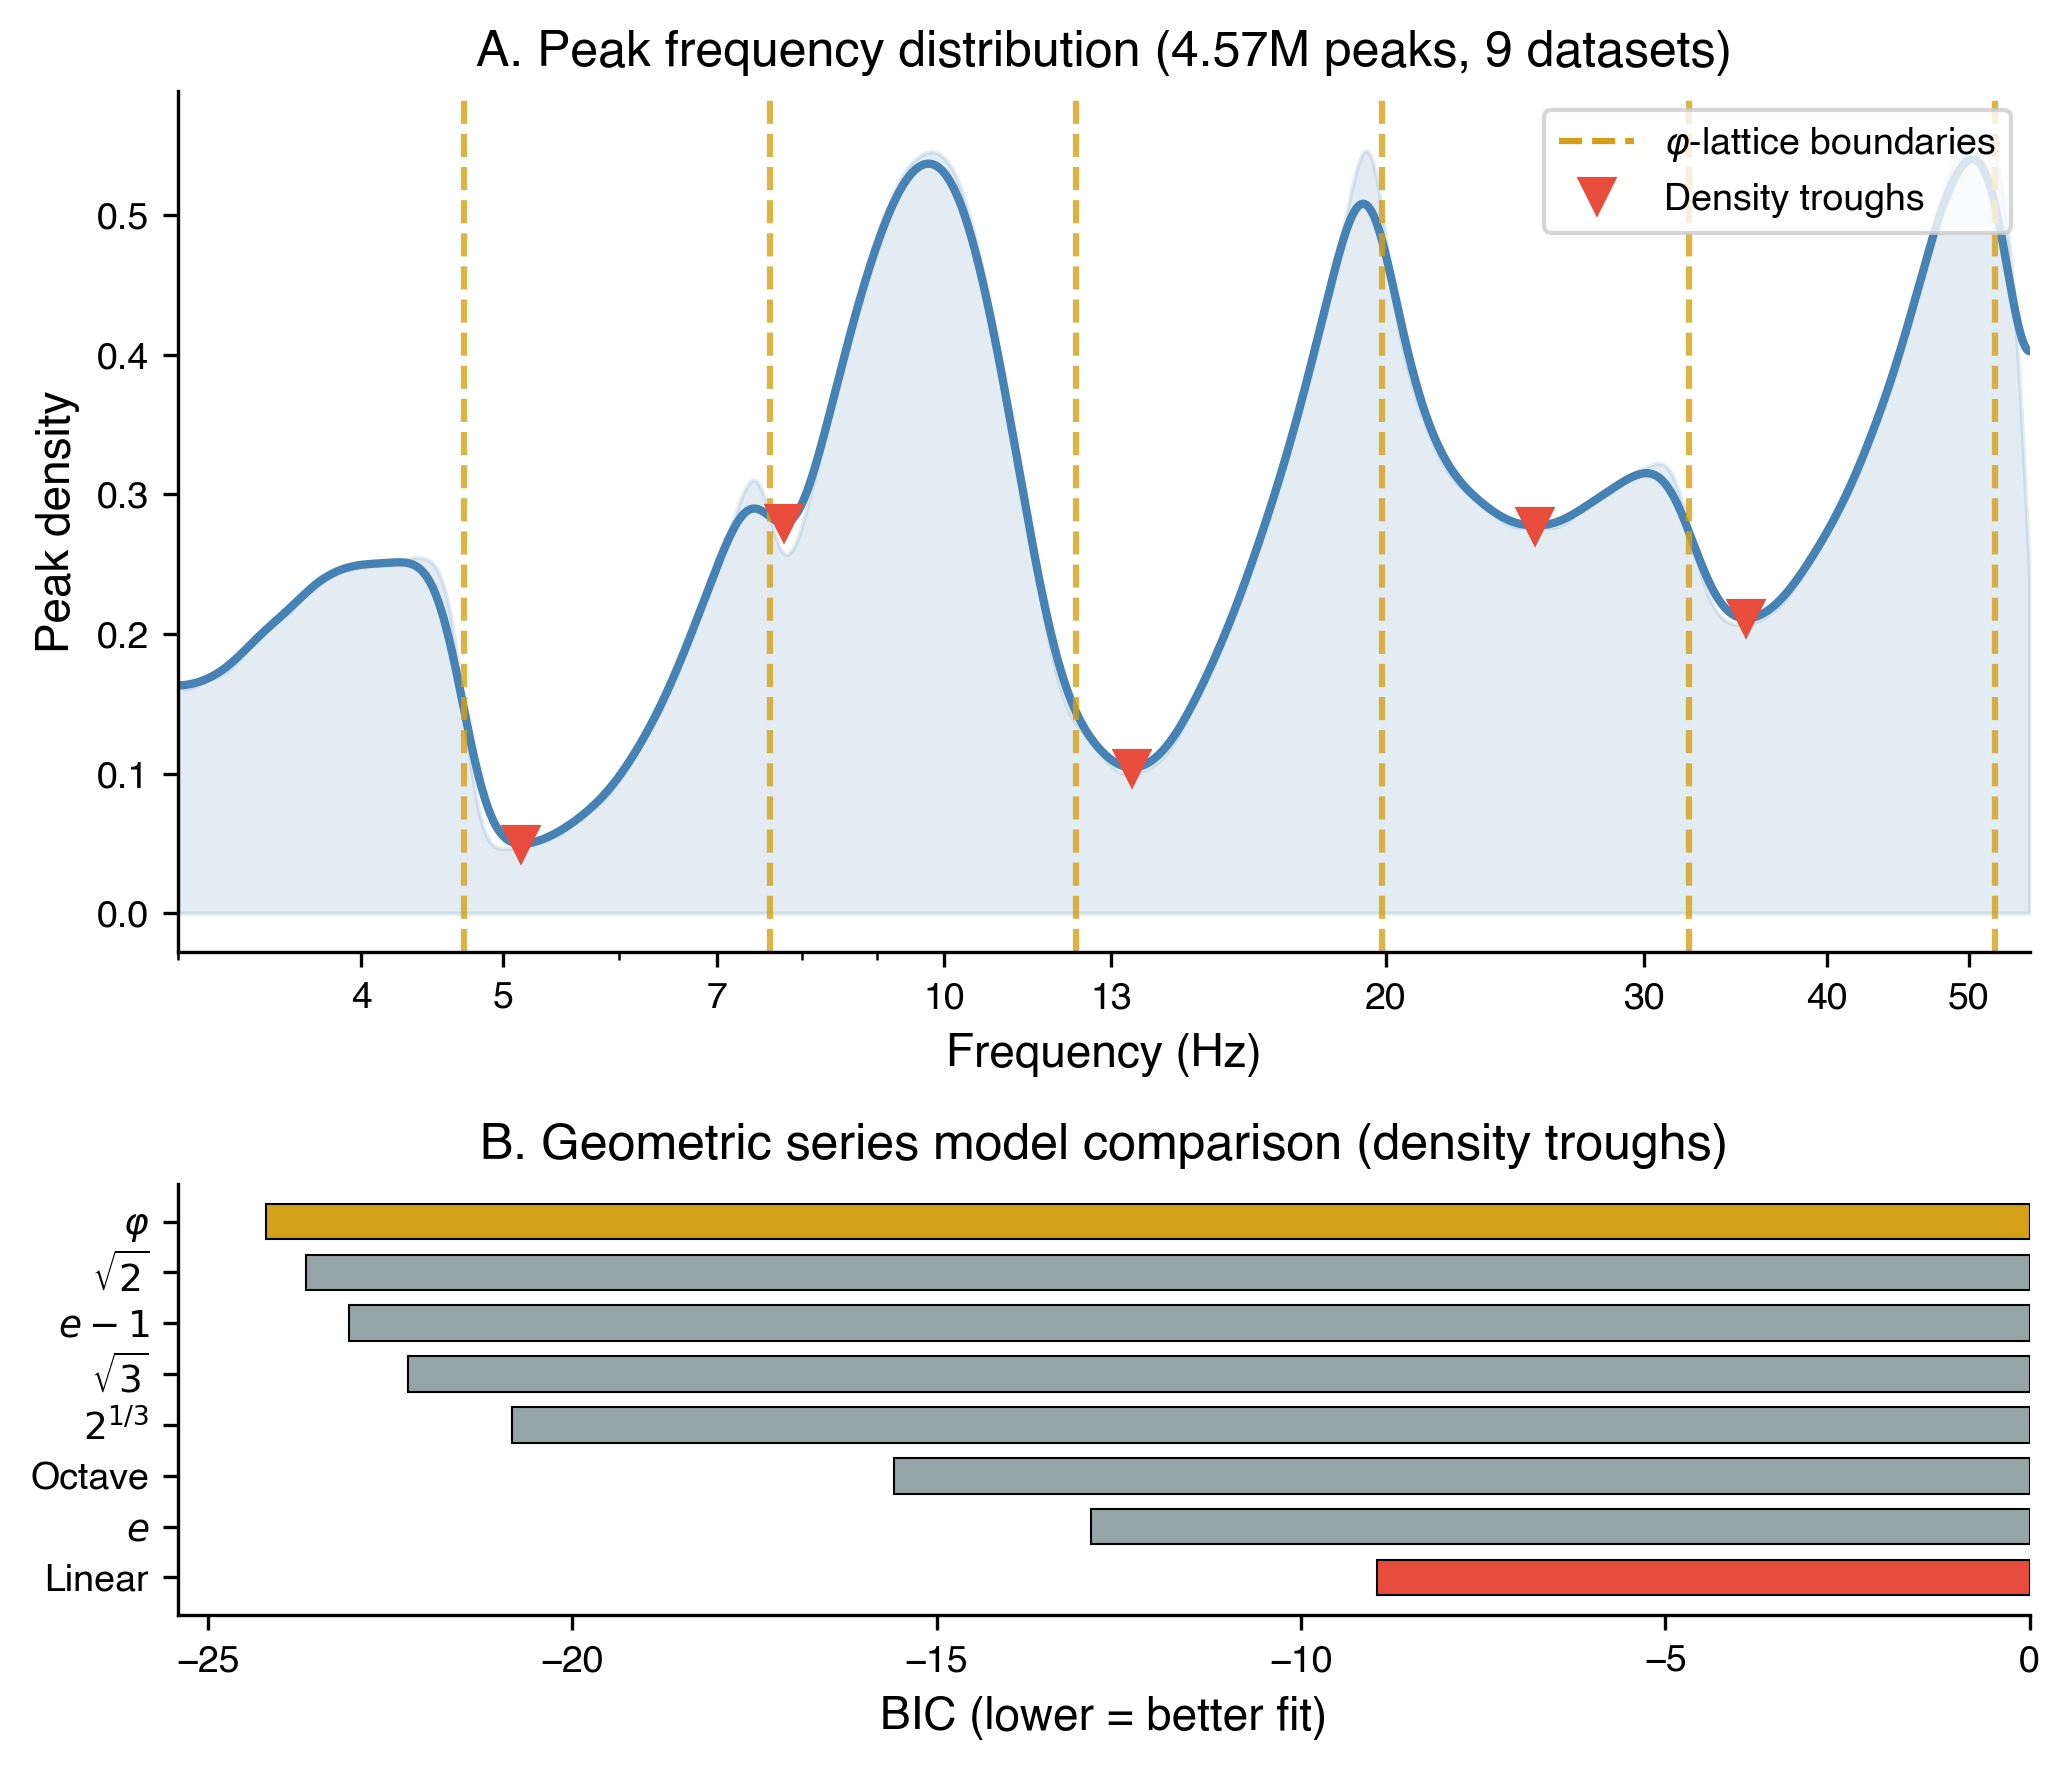
\includegraphics[width=\textwidth]{fig1_peak_density.png}
\caption{\textbf{Peak frequency distribution and model comparison.} (A)~Gaussian KDE of 4,572,489 FOOOF-detected peaks from $N = 2{,}097$ subjects (9 datasets) in log-Hz space. Gold dashed lines mark $\phisym$-lattice boundaries ($\fzero \times \phisym^n$); red triangles mark empirical density troughs. The geometric mean ratio of consecutive troughs is 1.6175, indistinguishable from $\phisym = 1.618$. (B)~Bayesian Information Criterion (BIC) comparison of geometric series models fit to trough positions (least-squares in log-frequency space, 1 free parameter per fixed-ratio model, 2 for the free-ratio model). $\phisym$ achieves the lowest BIC ($-24.2$); linear spacing is excluded by $\Delta$BIC $> 15$.}
\label{fig:peak_density}
\end{figure}

\begin{figure}[htbp]
\centering
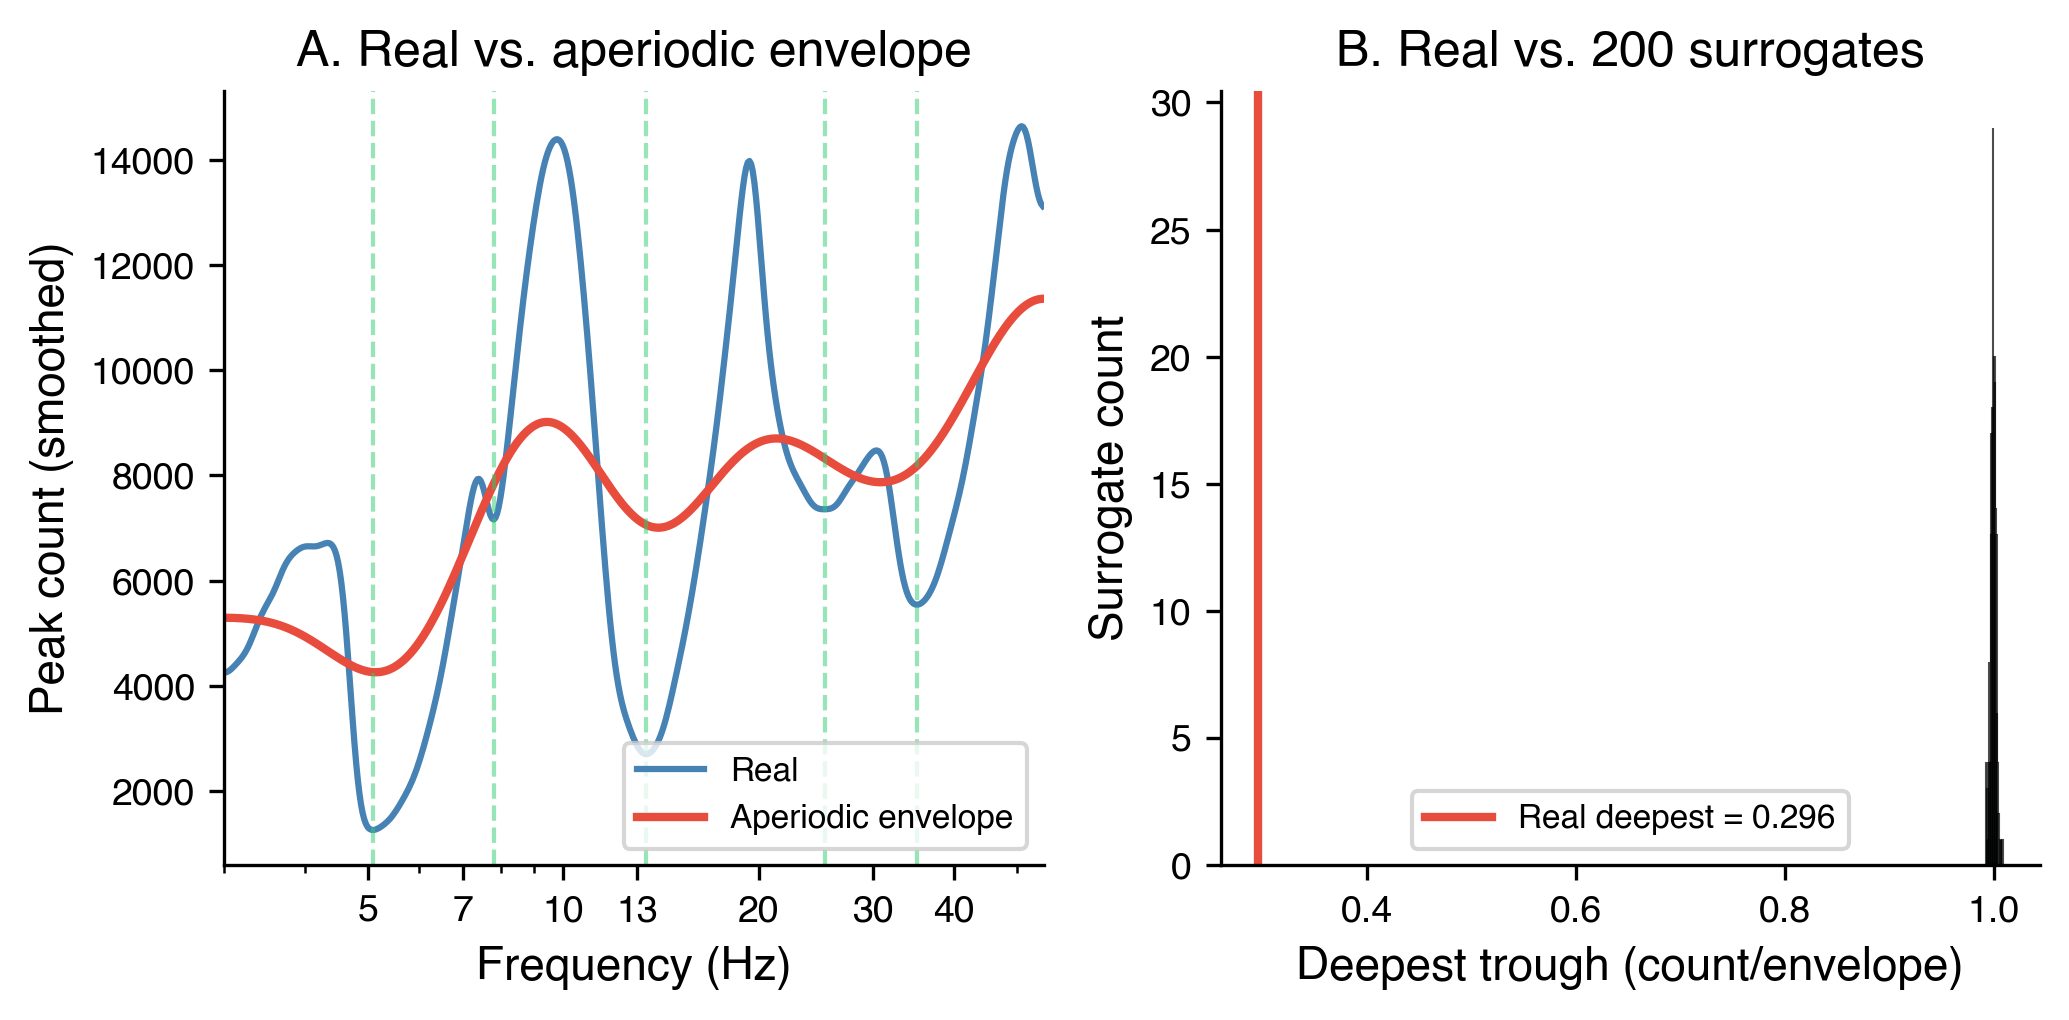
\includegraphics[width=\textwidth]{fig2_aperiodic_null.png}
\caption{\textbf{Aperiodic-only null test.} (A)~Real peak density (blue, $N = 4{,}572{,}489$ peaks) versus the smooth aperiodic envelope (red) obtained by heavy Gaussian smoothing ($\sigma = 40$ bins on 1,000-bin log-frequency histogram). Green dashed lines mark the five empirical troughs. (B)~Distribution of the deepest trough depth across 200 Poisson surrogates drawn from the aperiodic envelope. The real deepest trough (depth ratio $= 0.296$, red line) lies far outside the surrogate distribution (surrogate mean $= 1.004 \pm 0.004$ SD; permutation test, $p < 0.0001$), confirming that density troughs reflect genuine band structure, not $1/f$ artefacts.}
\label{fig:aperiodic_null}
\end{figure}

\subsubsection{Boundaries are Stable Across Smoothing Parameters}
\label{sec:stability}

The number and location of detectable troughs in a kernel density estimate depends on the smoothing bandwidth---over-smoothed estimates merge nearby troughs, while under-smoothed estimates fragment genuine troughs into noise. A robust boundary must survive across a wide range of smoothing levels.

We computed trough locations across 30 smoothing bandwidths ($\sigma = 2$--30 bins on the 1000-bin log-frequency histogram). Three troughs survive the full range of smoothing levels: $5.18 \pm 0.17$ Hz (30/30 smoothings), $13.44 \pm 0.05$ Hz (30/30), and $25.29 \pm 0.40$ Hz (24/30). These are the most bandwidth-robust troughs---features that no choice of smoothing can eliminate. Additional troughs at approximately 7.6 Hz and 35 Hz emerge at narrow smoothing bandwidths ($\sigma < 8$ bins) but merge into adjacent features at wider smoothings. All five troughs are confirmed genuine by the aperiodic null (Section~\ref{sec:boundaries_genuine}).

Note that bandwidth stability and trough depth measure different properties. The $\sim$35 Hz trough is deeper than the $\sim$25 Hz trough (32\% vs.\ 12\% depletion; Table~\ref{tab:aperiodic_null}) and is therefore more reliably detected in individual datasets (Section~\ref{sec:goldenratio}), but the $\sim$25 Hz trough is more stable across smoothing bandwidths. Both are genuine spectral features. The full dataset thus exhibits \emph{hierarchical trough structure}: five boundaries whose inter-trough geometric mean ratio is $\phisym$, with the two shallowest ($\sim$7.6 Hz and $\sim$25 Hz) detectable only at narrow smoothing or large pooled sample sizes. The pooled density is used throughout Part~I to estimate \emph{population geometry}---the positions, depths, and scaling of band boundaries---not to imply that each individual expresses the full five-trough structure with equal clarity. Per-dataset analyses resolve the three coarsest troughs; the two shallower boundaries require pooling for detection, reflecting their dependence on large samples rather than any artefact of pooling. The subject-level bootstrap (Section~\ref{sec:bootstrap}) directly addresses the dependence structure by resampling subjects rather than peaks.

\subsubsection{The Golden Ratio Best Fits Empirical Boundaries}
\label{sec:goldenratio}

Kernel density estimation of all 4,572,489 pooled peaks identifies five density troughs at 5.15, 7.77, 13.43, 25.29, and 35.24 Hz. Consecutive ratios between adjacent troughs are 1.510, 1.728, 1.883, and 1.393. The geometric mean of these four ratios is \textbf{1.6175}, indistinguishable from the golden ratio $\phisym = 1.6180$ to three significant figures.

To determine which candidate scaling ratio best accounts for these boundaries, we fit geometric series models $f_k = \fzero \times r^k$ for seven candidate values of $r$, optimising $\fzero$ by least-squares in log-frequency space (1 free parameter per model), and also tested a free-ratio model (2 free parameters) and linear-Hz spacing (2 parameters). Models were compared by BIC (Table~\ref{tab:model_comparison}).

\begin{table}[h]
\centering
\caption{Model comparison for geometric series fits to empirical density troughs (upper panel) and density peaks (lower panel). BIC is computed with the number of free parameters in parentheses; lower BIC indicates better fit. Mean error is in cents (100 cents = 1 semitone).}
\label{tab:model_comparison}
\begin{threeparttable}
\begin{tabular}{l r r r r r}
\toprule
Model & Ratio $r$ & Optimal $\fzero$ (Hz) & SSE & BIC & Mean error (cents) \\
\midrule
\multicolumn{6}{l}{\textit{Fitting to density troughs (5 boundaries)}} \\
\midrule
$\phisym$ & 1.618 & 5.23 & 0.0257 & $\mathbf{-24.74}$ & \textbf{93} \\
$\sqrt{2}$ & 1.414 & 6.84 & 0.0354 & $-23.14$ & 132 \\
$e - 1$   & 1.718 & 4.63 & 0.0360 & $-23.06$ & 124 \\
$\sqrt{3}$ & 1.732 & 4.56 & 0.0428 & $-22.20$ & 129 \\
$2^{1/3}$ & 1.260 & 9.90 & 0.0557 & $-20.88$ & 140 \\
Octave    & 2.000 & 3.93 & 0.1582 & $-15.66$ & 267 \\
$e$       & 2.718 & 11.20 & 0.2720 & $-12.95$ & 381 \\
Linear-Hz & ---   & ---  & 0.4139 & $-9.24$  & --- \\
Free ratio\tnote{a} & 1.366 & 10.01 & 0.0057 & $-30.69$ & --- \\
\midrule
\multicolumn{6}{l}{\textit{Fitting to density peaks (5 band centres)}} \\
\midrule
$\phisym$ & 1.618 & 6.94 & 0.0287 & $\mathbf{-24.20}$ & 105 \\
$\sqrt{2}$ & 1.414 & 7.41 & 0.0306 & $-23.87$ & 106 \\
$e - 1$   & 1.718 & 3.80 & 0.0571 & $-20.75$ & 164 \\
$2^{1/3}$ & 1.260 & 7.76  & 0.0627 & $-20.29$ & 140 \\
$\sqrt{3}$ & 1.732 & 11.23 & 0.0663 & $-20.00$ & 180 \\
Octave    & 2.000 & 4.25 & 0.0682 & $-19.87$ & 181 \\
$e$       & 2.718 & 9.19 & 0.2026 & $-14.42$ & 327 \\
Linear-Hz & ---   & ---  & 0.4971 & $-8.32$  & --- \\
Free ratio\tnote{a} & 1.334 & 7.50 & 0.0098 & $-27.94$ & --- \\
\bottomrule
\end{tabular}
\begin{tablenotes}
\small
\item[a] Free-ratio model optimises both $\fzero$ and $r$ (2 free parameters).
\end{tablenotes}
\end{threeparttable}
\end{table}

Four findings are clear. First, linear-Hz spacing is excluded with decisive force: $\Delta$BIC $= 15.5$ versus $\phisym$ for troughs, 15.9 for peaks. Second, Euler's number $e$ is strongly excluded (BIC $= -12.95$ vs. $-24.74$ for $\phisym$; $\Delta$BIC $= 11.8$). The \textcite{penttonen2003natural} claim that the inter-band ratio is $\approx e$ is not supported in unbiased peak data. Third, $\phisym$ is the best single fixed-ratio model for both boundary positions (BIC $= -24.74$) and band centres (BIC $= -24.20$), with a mean error of 93 cents (less than one semitone) for troughs. For band centres, $\sqrt{2}$ is close to $\phisym$ (BIC $-23.87$ vs. $-24.20$; $\Delta$BIC $= 0.3$, negligible). Fourth, the discrimination among the three leading candidates---$\phisym$ (1.618), $\sqrt{2}$ (1.414), and $e - 1$ (1.718)---is not sharp: BIC differences of 0.1--1.7 are meaningful but not decisive. All three describe the data far better than any octave-family ratio.

Per-dataset replication yields a different picture. Analysing each of the 9 datasets independently, trough detection reliably finds 2--4 troughs per dataset (typically at $\sim$5.5, $\sim$13.5, and $\sim$35 Hz), with an overall geometric mean ratio of 2.060 (log-SD 0.231). One-sample $t$-tests against candidate constants with $N = 24$ ratios reject $\phisym$ ($t_{23} = +5.02$, $p < 0.001$), $e - 1$ ($p = 0.001$), and $e$ ($p < 0.001$), but cannot reject the octave ratio 2.0 ($t_{23} = +0.61$, $p = 0.548$). This is not a contradiction with the pooled result: individual datasets reliably detect only the three deepest troughs---at $\sim$5, $\sim$13, and $\sim$35 Hz---which are the most depleted boundaries (70\%, 62\%, and 32\% depletion respectively; Table~\ref{tab:aperiodic_null}). These three span ratios of $\sim$2.5, biased toward the octave. The pooled 5-trough solution additionally resolves the two shallower boundaries at $\sim$7.6 Hz (9\% depletion) and $\sim$25 Hz (12\% depletion) that per-dataset analysis misses at typical sample sizes, and those finer boundaries reduce the geometric mean ratio to $\phisym$. The per-dataset octave finding and the pooled $\phisym$ finding are two views of the same hierarchical structure described in Section~\ref{sec:stability}. Crucially, the subject-level bootstrap (Section~\ref{sec:bootstrap}) recovers all five troughs---including the two shallower boundaries at $\sim$7.6 and $\sim$25~Hz---in 100\% of 1,000 iterations, confirming that these finer boundaries are population-level realities detectable with proper dependence-aware resampling, not pooling artifacts that vanish at per-dataset resolution.

\subsubsection{Subject-Level Bootstrap Validates the Five-Trough Solution}
\label{sec:bootstrap}

The preceding analyses pool 4,572,489 peaks and treat them as independent observations. Because peaks are nested within subjects, sessions, and channels, the effective sample size for trough estimation is substantially lower, and confidence intervals from pooled analyses may be artificially narrow. To address this, we performed a stratified bootstrap over subjects: at each of 1,000 iterations, subjects were resampled with replacement independently within each of the 9 datasets (preserving dataset composition), their peaks were pooled, and the full trough-detection pipeline was re-run from scratch.

All five troughs were recovered in 100\% of bootstrap iterations. Position CIs were tight: the $\fzero$ boundary at 7.82~Hz was localized to within $\pm 0.015$~Hz; even the broadest CI (trough 4 at 24.75~Hz: [24.25, 26.01]) spans only 1.75~Hz (Table~\ref{tab:bootstrap_ci}).

\begin{table}[h]
\centering
\caption{Subject-level bootstrap confidence intervals for density trough positions. $N = 2{,}097$ subjects, 1,000 stratified bootstrap iterations. All five troughs detected in 100\% of iterations.}
\label{tab:bootstrap_ci}
\begin{tabular}{r r r r}
\toprule
Trough & Hz & 95\% CI & Width (Hz) \\
\midrule
1 & 5.03  & [4.98, 5.13]   & 0.15 \\
2 & 7.82  & [7.82, 7.85]   & 0.02 \\
3 & 13.59 & [13.40, 13.83] & 0.44 \\
4 & 24.75 & [24.25, 26.01] & 1.75 \\
5 & 34.38 & [34.18, 34.79] & 0.60 \\
\bottomrule
\end{tabular}
\end{table}

The bootstrap distribution of the global inter-trough geometric mean ratio had median 1.617 and 95\% CI [1.609, 1.623] (SD $= 0.004$). Of the candidate constants discussed in the literature (Figure~\ref{fig:bootstrap}):

\begin{itemize}
    \item $\phisym = 1.618$: \textbf{within the CI} ($p = 0.90$)
    \item $e - 1 = 1.718$: excluded ($p < 0.0001$)
    \item $\sqrt{2} = 1.414$: excluded ($p < 0.0001$)
    \item $\sqrt{3} = 1.732$: excluded ($p < 0.0001$)
    \item Octave $= 2.0$: excluded ($p < 0.0001$)
    \item $e = 2.718$: excluded ($p < 0.0001$)
\end{itemize}

The subject-level bootstrap resolves the ambiguity left by the BIC analysis: when the dependence structure is properly accounted for, the 95\% CI on the global scaling ratio spans only 0.014 and contains $\phisym$ while excluding every other named candidate. This does not imply that each adjacent boundary pair is individually $\phisym$-spaced---the local ratios remain heterogeneous (1.36--1.89)---but it establishes that $\phisym$ is the best-supported named global coordinate constant among the theoretical alternatives tested.

\begin{figure}[htbp]
\centering
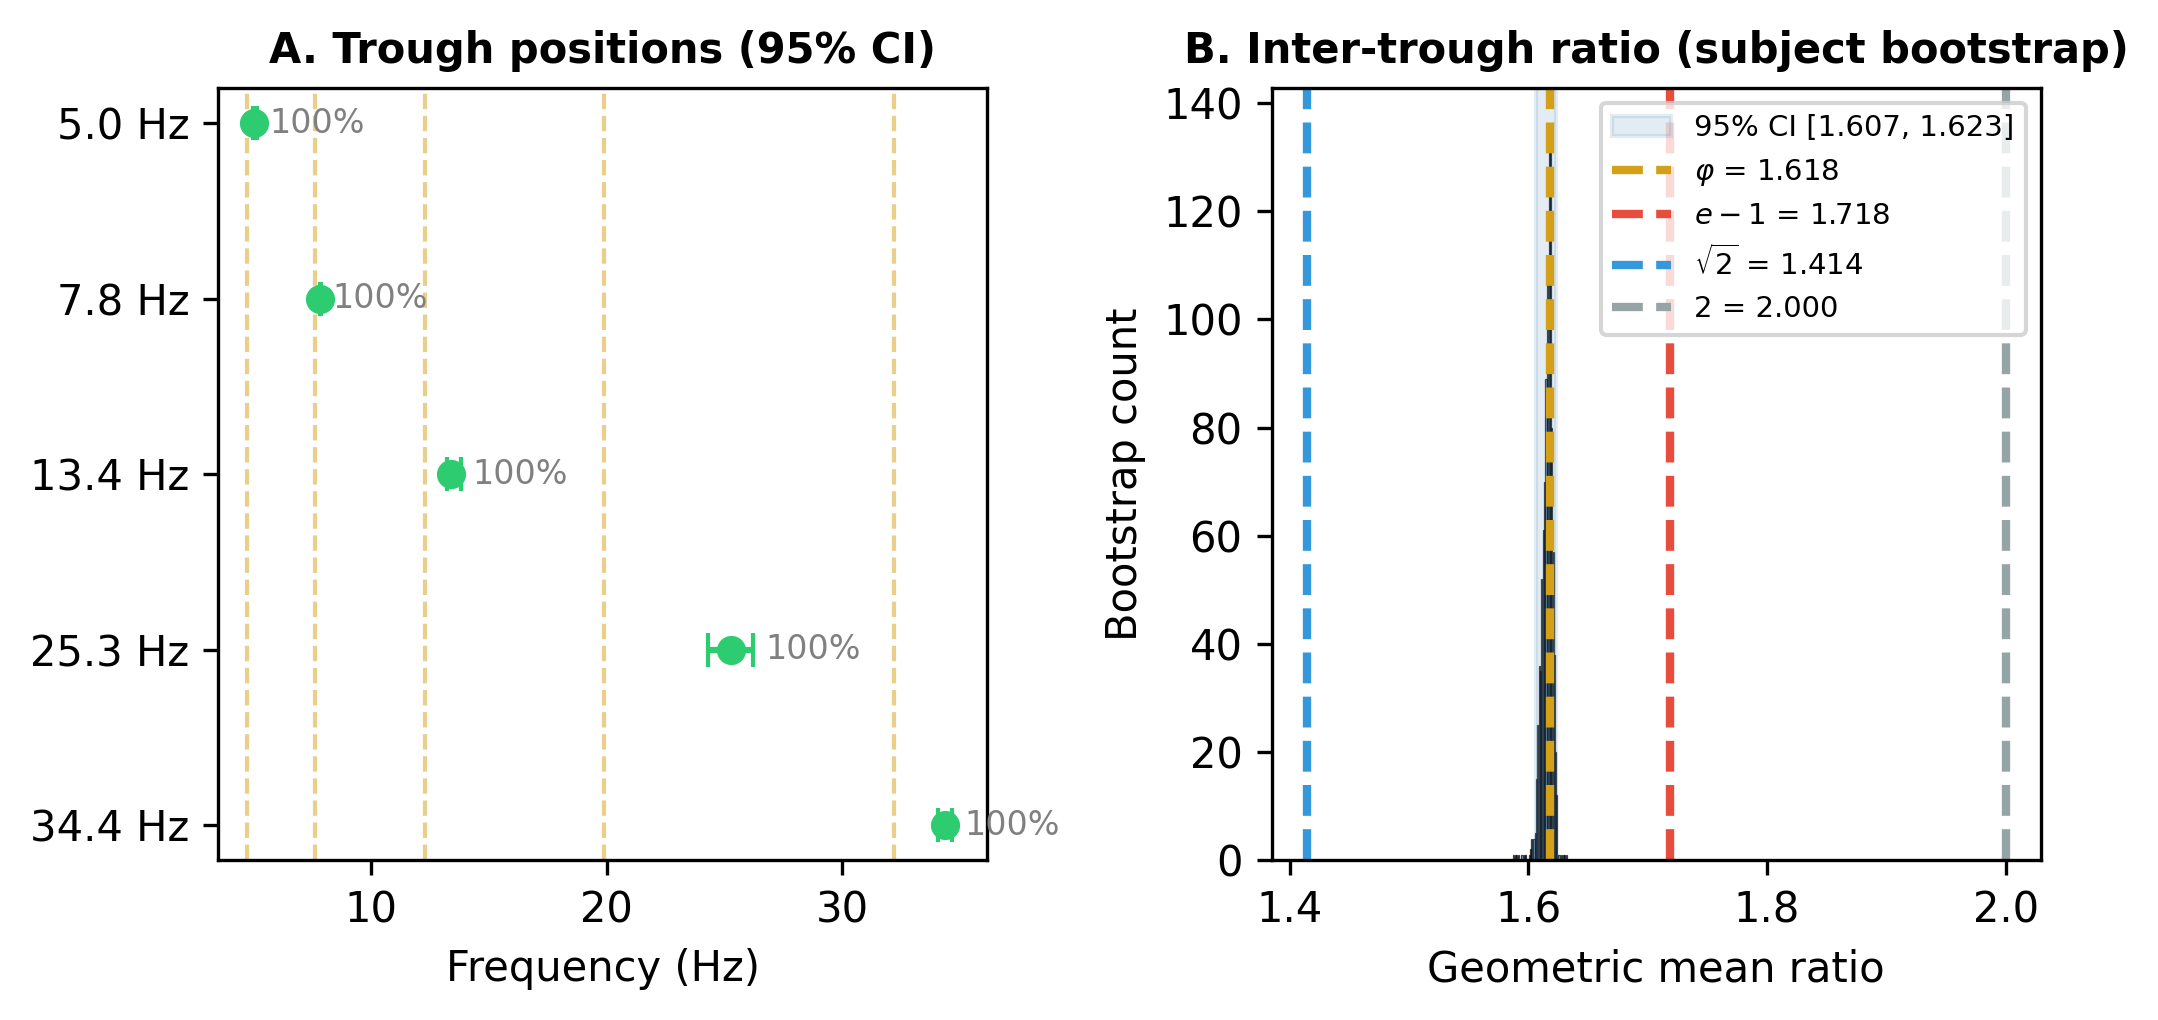
\includegraphics[width=\textwidth]{fig9_bootstrap.png}
\caption{\textbf{Subject-level bootstrap of trough positions and inter-trough ratio.} (A)~95\% confidence intervals for each of five density trough positions, computed from 1,000 stratified bootstrap resamples over $N = 2{,}097$ subjects (resampled with replacement within each of 9 datasets). Gold dashed lines mark $\phisym$-lattice boundaries. Percentages indicate detection rate (100\% for all troughs). Error bars show 2.5th--97.5th percentile bootstrap CIs. (B)~Bootstrap distribution of the global geometric mean ratio of consecutive trough frequencies (SD $= 0.004$). The 95\% CI [1.609, 1.623] (shaded) contains $\phisym = 1.618$ (gold, two-tailed permutation $p = 0.90$) and excludes all other named candidates (all $p < 0.0001$).}
\label{fig:bootstrap}
\end{figure}

\subsubsection{$\phisym$-Lattice Boundaries are Near-Optimal}
\label{sec:boundaries}

The BIC analysis establishes $\phisym$ as the best fixed-ratio model for empirical boundaries. A separate question is whether the specific boundary \emph{positions} produced by the $\phisym$-lattice ($\fzero \times \phisym^n$ with $\fzero = 7.60$ Hz) are optimal for measurement purposes---that is, whether they produce simple, consistent within-band enrichment profiles. We assess this with a boundary sweep.

A $36 \times 36$ grid of $(\fzero, r)$ pairs spanning $\fzero \in [6.0, 9.5]$ Hz and $r \in [1.3, 2.3]$ was evaluated. For each coordinate system, within-band enrichment profiles were computed and their simplicity measured by the $R^2$ of a low-order polynomial fit. Among all named systems tested (Table~\ref{tab:boundary_sweep}), the $\phisym$-lattice achieves the highest profile simplicity ($R^2 = 0.968$)---enrichment profiles within each band are nearly perfectly described by low-order polynomials when boundaries are placed at $\fzero \times \phisym^n$.

\begin{table}[h]
\centering
\caption{Named boundary systems evaluated in the $36 \times 36$ coordinate sweep.
Profile simplicity is the mean $R^2$ of a low-order polynomial fit to within-band enrichment profiles (higher = simpler, more interpretable profiles). Cross-dataset consistency is the mean pairwise Pearson $r$ of enrichment vectors across 9 datasets.}
\label{tab:boundary_sweep}
\begin{tabular}{l r r r}
\toprule
System & Ratio & Simplicity $R^2$ & Consistency $r$ \\
\midrule
$\phisym$-lattice  & 1.618 & \textbf{0.968} & 0.802 \\
Third-octave       & 1.260 & 0.942          & \textbf{0.896} \\
$\sqrt{2}$         & 1.414 & 0.886          & 0.677 \\
Clinical (4--8--13--30 Hz) & $\sim$1.63 & 0.807 & 0.808 \\
Octave             & 2.000 & 0.647          & 0.819 \\
\bottomrule
\end{tabular}
\end{table}

A boundary slide analysis tested whether each of the four $\phisym$-lattice boundaries is individually near-optimal for profile simplicity (i.e., measurement-optimal, not biologically optimal in any demonstrated sense). Each boundary was independently varied $\pm 25\%$ from its $\phisym$-lattice position while holding the others fixed. All four boundaries lie within 2\% of their simplicity-maximising positions (Table~\ref{tab:boundary_slide}). The theta/alpha boundary at $\fzero = 7.60$ Hz is exactly at the optimum (0.0\% offset).

\begin{table}[h]
\centering
\caption{Boundary slide analysis: optimal boundary positions for profile simplicity relative to $\phisym$-lattice positions.}
\label{tab:boundary_slide}
\begin{tabular}{l r r r}
\toprule
Boundary & $\phisym$-lattice (Hz) & Optimal (Hz) & Offset \\
\midrule
$\theta / \alpha$              & 7.60  & \textbf{7.60}  & \textbf{0.0\%} \\
$\alpha / \beta_{\text{low}}$  & 12.30 & 12.05          & $-2.0\%$ \\
$\beta_{\text{low}} / \beta_{\text{high}}$ & 19.90 & 20.10 & $+1.0\%$ \\
$\beta_{\text{high}} / \gamma$ & 32.19 & 32.52          & $+1.0\%$ \\
\bottomrule
\end{tabular}
\end{table}

\begin{figure}[htbp]
\centering
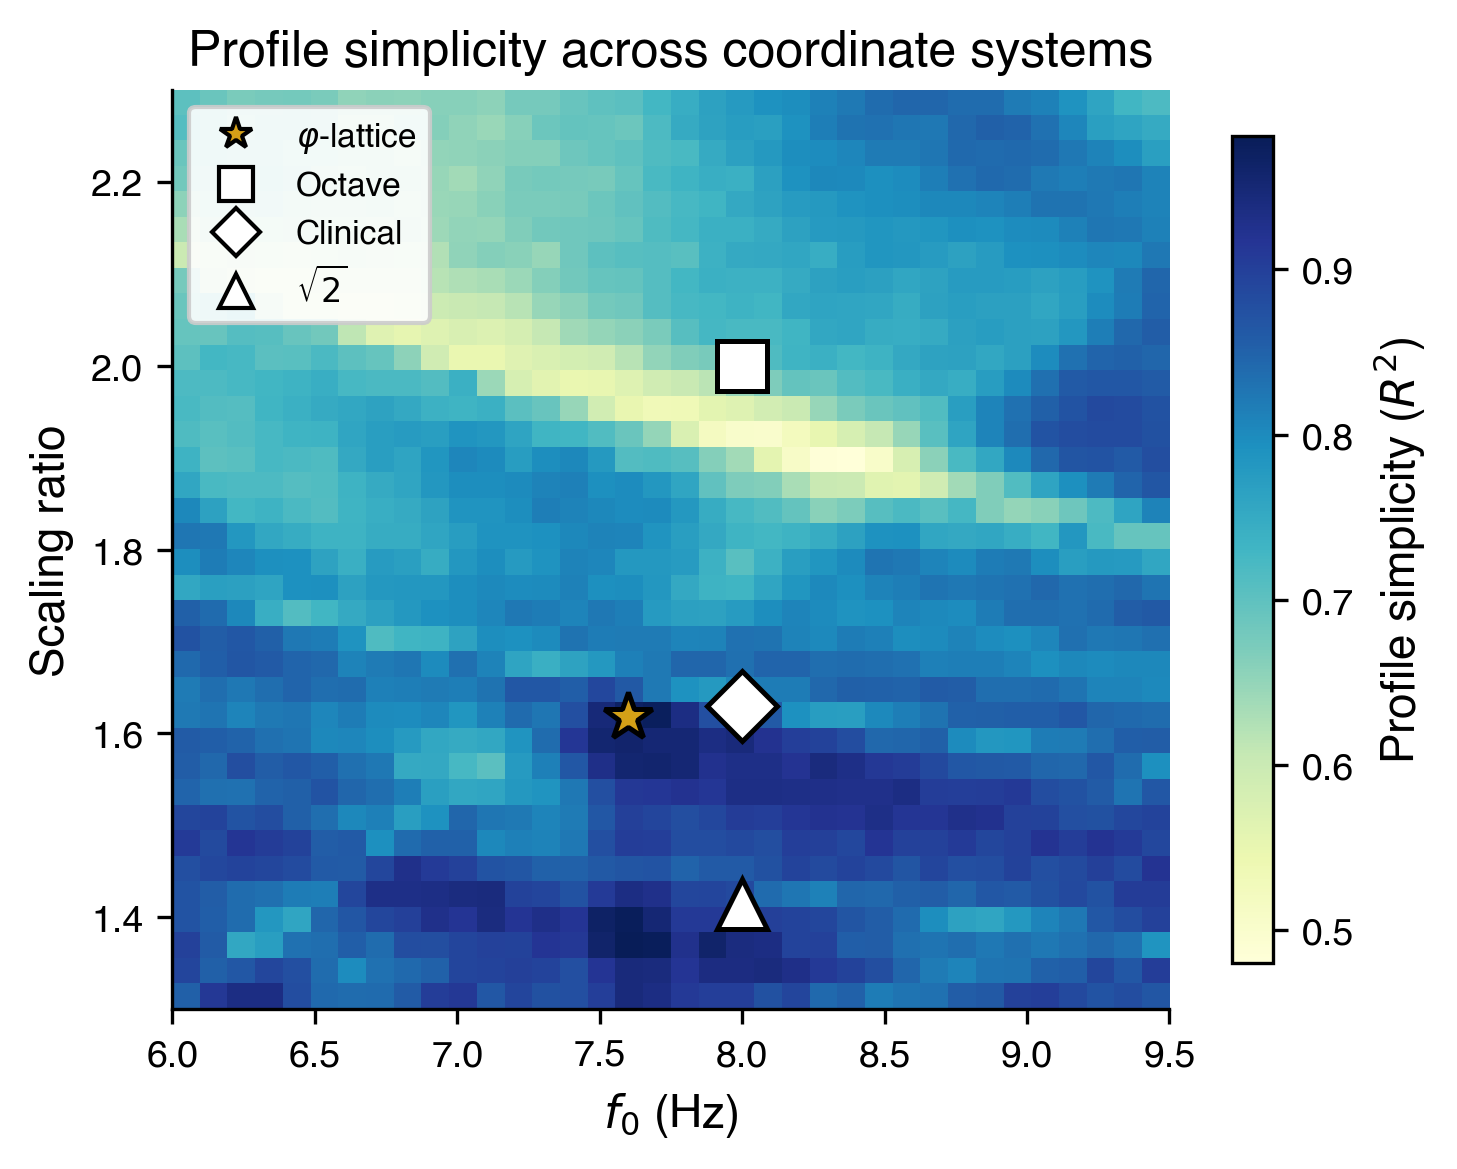
\includegraphics[width=0.7\textwidth]{fig3_boundary_sweep.png}
\caption{\textbf{Boundary sweep: profile simplicity across coordinate systems.} Heatmap of within-band profile simplicity (mean $R^2$ of low-order polynomial fits to enrichment profiles) across a $36 \times 36$ grid of 1,296 $(\fzero, r)$ coordinate systems, evaluated on 4.57 million peaks from $N = 2{,}097$ subjects. The $\phisym$-lattice (gold star) achieves the highest simplicity ($R^2 = 0.968$). Other named systems are marked for comparison: octave (square), clinical convention (diamond), $\sqrt{2}$ (triangle).}
\label{fig:boundary_sweep}
\end{figure}

\paragraph{Summary.} At the population level, the data support log-frequency organisation unequivocally ($\Delta$BIC $> 46$); support a $\phisym$-like global coordinate constant among named alternatives (bootstrap 95\% CI [1.609, 1.623]); and do \emph{not} support special within-band $\phisym$ landmarks (noble-number positions carry no more signal than simple rationals). The $\phisym$-lattice is a measurement-optimal coordinate system---its value is boundary placement for revealing simple enrichment profiles, not a claim about golden-ratio computation in neural circuits.

\subsubsection{Within Bands, No Fine-Structure at $\phisym$-Specific Positions}
\label{sec:within}

The $\phisym$-lattice places not only boundaries but also interior landmarks within each band: noble numbers, inverse nobles, and the band attractor. These have been proposed as sites of privileged oscillatory activity \parencite{pletzer2010golden}, on the grounds that $\phisym$-irrational positions maximally resist synchronisation with other bands. We test this prediction directly.

Five analyses addressed whether $\phisym$-specific positions carry special signal within bands. First, a landmark capture test compared the enrichment variance explained by $\phisym$-lattice positions against equal-spaced positions and 1000 random position sets: $\phisym$-lattice positions ranked at the 55th--81st percentile of random sets---numerically better than average but not significantly so ($p > 0.05$ in all bands). Second, a feature alignment test asked whether enrichment extrema preferentially fall at $\phisym$ positions: in 3 of 4 testable bands, simple rational positions ($1/2$, $1/3$, $2/3$) were \emph{closer} to the extrema than $\phisym$ positions were. Third, a noble-versus-rational permutation test found no significant enrichment difference between noble numbers and simple rationals in any band ($p = 0.67$--$0.98$). Fourth, periodicity analysis found no sub-octave periodic structure in the within-band enrichment profiles: the dominant period in all bands is 1.0 (the full log-octave), with no harmonics at $1/\phisym$, $1/2$, or other sub-octave values.

Within-band enrichment profiles are smooth, low-dimensional curves---ascending ramps in theta, beta-low, and gamma; a descending ramp in beta-high; a single broad mountain in alpha---fully characterised by 2--3 parameters with no fine-structure at any mathematically special interior positions. The $\phisym$-lattice provides value through its boundary placement, not through any privileged significance of its interior coordinates.

\subsubsection{Relationship to Prior Work}

All results reported in this paper use the v3 extraction pipeline, which corrects three systematic biases identified in a prior report \parencite{lacy2026frontiers}. These corrections---a $\fzero$ alignment mismatch, a Hz-weighting error in the enrichment null hypothesis, and a split-FOOOF boundary artefact---are documented in detail in Section~\ref{sec:methods_corrections} (Methods). The most consequential correction reversed the beta-low boundary enrichment from $+101\%$ to $-33\%$, invalidating the previously reported U-shape profile. Five enrichment values changed sign. The implications for the prior paper's claims are discussed in Section~3.6.


%------------------------------------------------------------------------------
\subsection{Part II: The Enrichment Landscape}
%------------------------------------------------------------------------------

\subsubsection{Two Organizational Regimes}
\label{sec:two-regimes}

Across 9 datasets and 2,097 subjects, the $\phisym$-lattice enrichment landscape resolves into two mutually exclusive organizational regimes. The first, \textit{Alpha Mountain}, is defined by enrichment concentrated in the central octave: the attractor position ($u = 0.500$, $\approx$9.67 Hz) reaches $+41\%$, Noble$_1$ ($u = 0.618$, $\approx$10.23 Hz) reaches $+30\%$, and inv\_noble$_1$ ($u = 0.382$, $\approx$9.13 Hz) reaches $+36\%$. Both octave boundaries are depleted (lower boundary $-35\%$, upper boundary $-73\%$). This mountain profile is the empirical realization of individual alpha frequency (IAF) clustering, reflecting thalamocortical T-type Ca$^{2+}$ channel dynamics with an intrinsic $\approx$100 ms time constant that pins oscillatory peaks to the mid-octave region independent of cortical frequency-gradient forces.

The second regime, \textit{Edge Ramp}, governs theta, beta-low, and gamma, in which peaks deplete across the lower octave and accumulate monotonically toward the upper octave boundary. In beta-low, the ramp spans from noble$_4$ ($-54\%$) to inv\_noble$_6$ ($+87\%$). In theta, the ramp is the steepest of any band, rising from the lower boundary ($-52\%$) to boundary\_hi ($+123\%$)---the latter representing $\fzero$ convergence under resting conditions. Beta-high exhibits the mirror pattern: a descending ramp from its lower boundary ($+85\%$) to boundary\_hi ($-18\%$), reflecting the same $\approx$20 Hz accumulation zone viewed from the opposing octave.

Profile consistency, assessed as the fraction of positions that agree in sign direction across all 9 datasets, confirms that these regimes are robust: theta 12/13, alpha 10/13, beta-low 12/13, beta-high 4/13, and gamma 6/13 positions are consistent. The weaker consistency of beta-high under FOOOF likely reflects sensitivity of the parametric aperiodic model in this frequency range: replication with IRASA, a non-parametric aperiodic decomposition method \parencite{wen2016irasa,gerster2022irasa}, yields 13/13 cross-dataset consistency for beta-high with a steeper gradient (192 versus 113 percentage points; see Section~\ref{sec:irasa}). Gamma consistency remains weak under both methods, likely reflecting electromyographic and microsaccade artifact contamination that scalp EEG cannot fully resolve (gamma results throughout this paper should be interpreted with this caveat).

\begin{figure}[htbp]
\centering
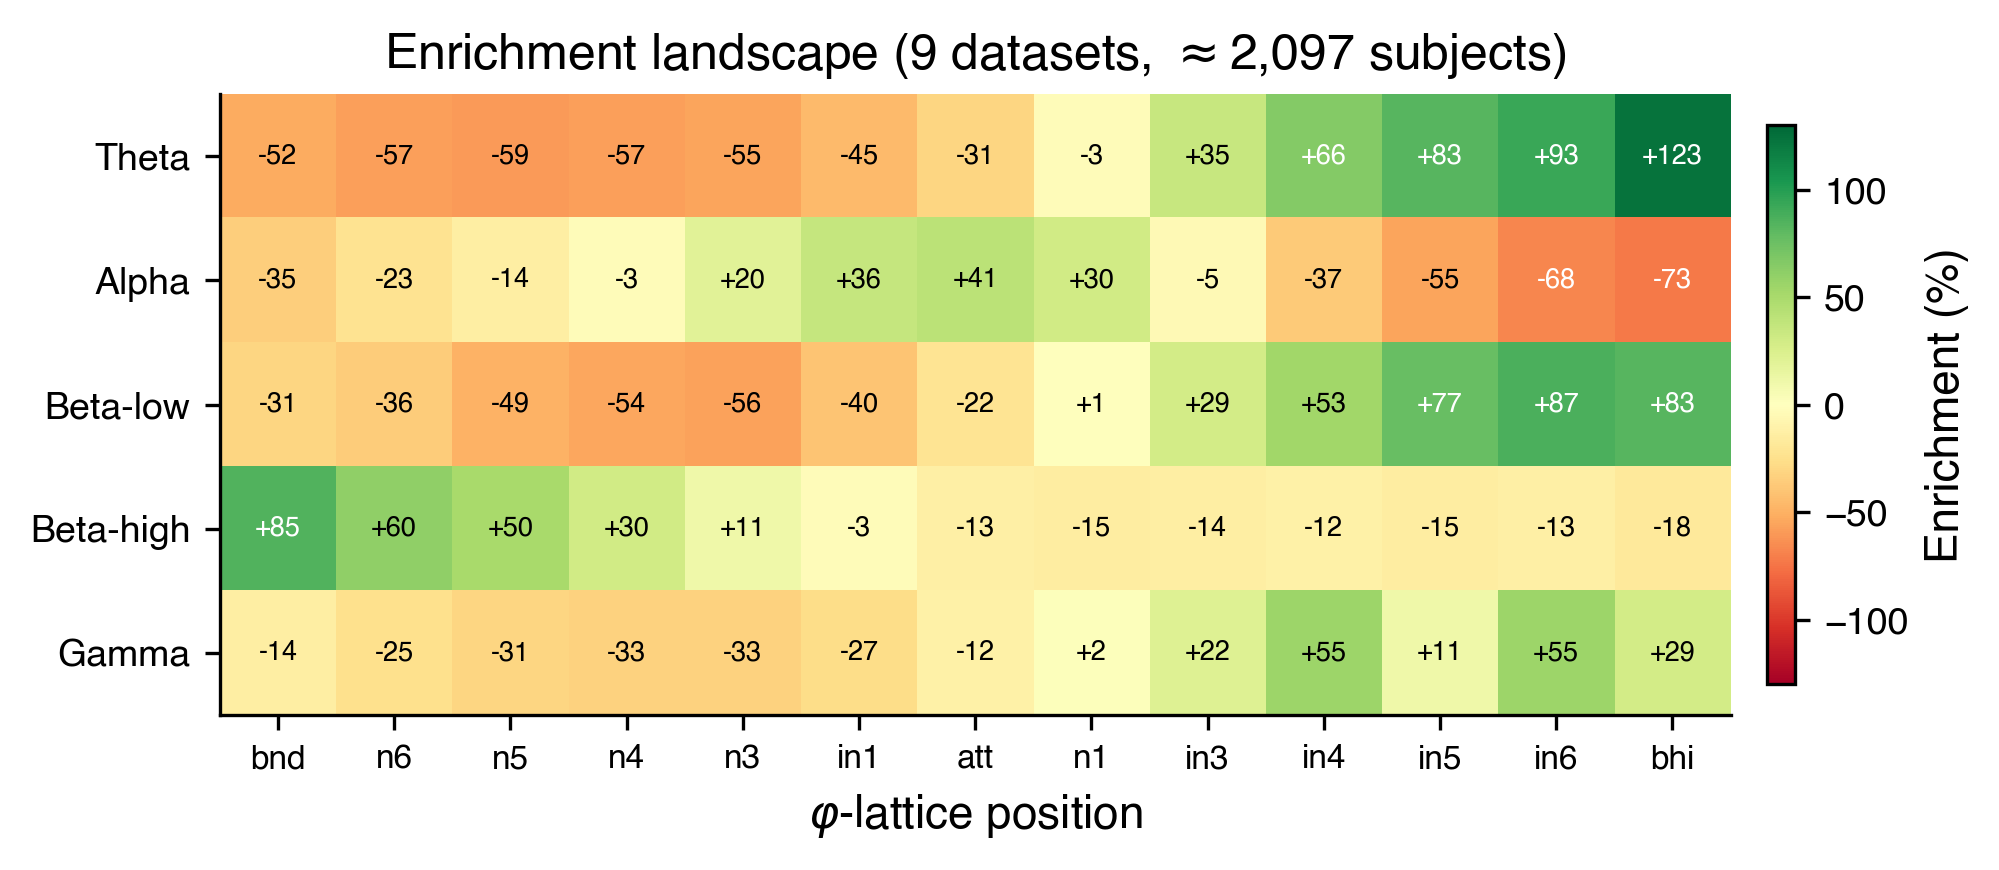
\includegraphics[width=\textwidth]{fig4_enrichment_landscape.png}
\caption{\textbf{Enrichment landscape across 5 frequency bands and 13 $\phisym$-lattice positions.} Values are means across 9 datasets ($N = 2{,}097$ subjects total, 4.57 million peaks; Hz-corrected Voronoi enrichment, top-50\% power filter). Green indicates enrichment (more peaks than expected under uniform log-frequency distribution); red indicates depletion. Alpha shows a central mountain (attractor $+43\%$); theta, beta-low, and gamma show ascending ramps; beta-high shows a descending ramp. The alpha profile is the approximate inverse of all other bands (Pearson $r \approx -0.95$ with theta across 13 positions).}
\label{fig:enrichment_landscape}
\end{figure}

\subsubsection{Cross-Boundary Architecture}
\label{sec:cross_boundaries}

The four $\phisym$-lattice band boundaries---located at $\fzero$, $\fzero \times \phisym$, $\fzero \times \phisym^2$, and $\fzero \times \phisym^3$---exhibit qualitatively distinct enrichment signatures (Table~\ref{tab:boundaries}). Each boundary type reflects a different interaction between the intrinsic dynamics of its flanking bands.

\begin{table}[h]
\centering
\caption{Cross-boundary enrichment architecture. Enrichment values are 9-dataset means, Hz-corrected, top-50\% power filter. $\Delta$ is the signed difference (above minus below). Boundary types: Cliff (sharp drop), Void (depleted both sides), Bridge (enriched both sides), Weak (near-null both sides).}
\label{tab:boundaries}
\begin{tabular}{lrrrrrl}
\toprule
\textbf{Boundary} & \textbf{Hz} & \textbf{$\phisym$-position} & \textbf{Below} & \textbf{Above} & \textbf{$\Delta$ (pp)} & \textbf{Type} \\
\midrule
$\theta / \alpha$       & 7.60  & $\fzero$              & $+123\%$ & $-35\%$ & $-158$ & Cliff  \\
$\alpha / \beta_{\mathrm{L}}$ & 12.30 & $\fzero \times \phisym$   & $-73\%$  & $-31\%$ & $+42$  & Void   \\
$\beta_{\mathrm{L}} / \beta_{\mathrm{H}}$ & 19.90 & $\fzero \times \phisym^2$ & $+83\%$  & $+85\%$ & $+2$   & Bridge \\
$\beta_{\mathrm{H}} / \gamma$ & 32.19 & $\fzero \times \phisym^3$ & $-18\%$  & $-14\%$ & $+4$   & Weak   \\
\bottomrule
\end{tabular}
\end{table}

The $\fzero$ boundary (7.60 Hz) is the sharpest spectral transition in the dataset: theta peaks accumulate at $+123\%$ immediately below while alpha begins at $-35\%$ immediately above, a discontinuity of $-158$ pp. The alpha/$\beta_{\mathrm{L}}$ boundary at 12.30 Hz is a spectral void, with both the upper flank of alpha ($-73\%$) and the lower flank of beta-low ($-31\%$) deeply depleted---a spectral desert spanning $\approx$11.5--13.2 Hz. The $\beta_{\mathrm{H}}$/$\gamma$ boundary at 32.19 Hz is functionally inert: both flanks are near zero ($-18\%$ below, $-14\%$ above). The $\beta_{\mathrm{L}}/\beta_{\mathrm{H}}$ boundary at 19.90 Hz is the sole exception to this pattern and is described in detail in Section~\ref{sec:bridge}.

\begin{figure}[htbp]
\centering
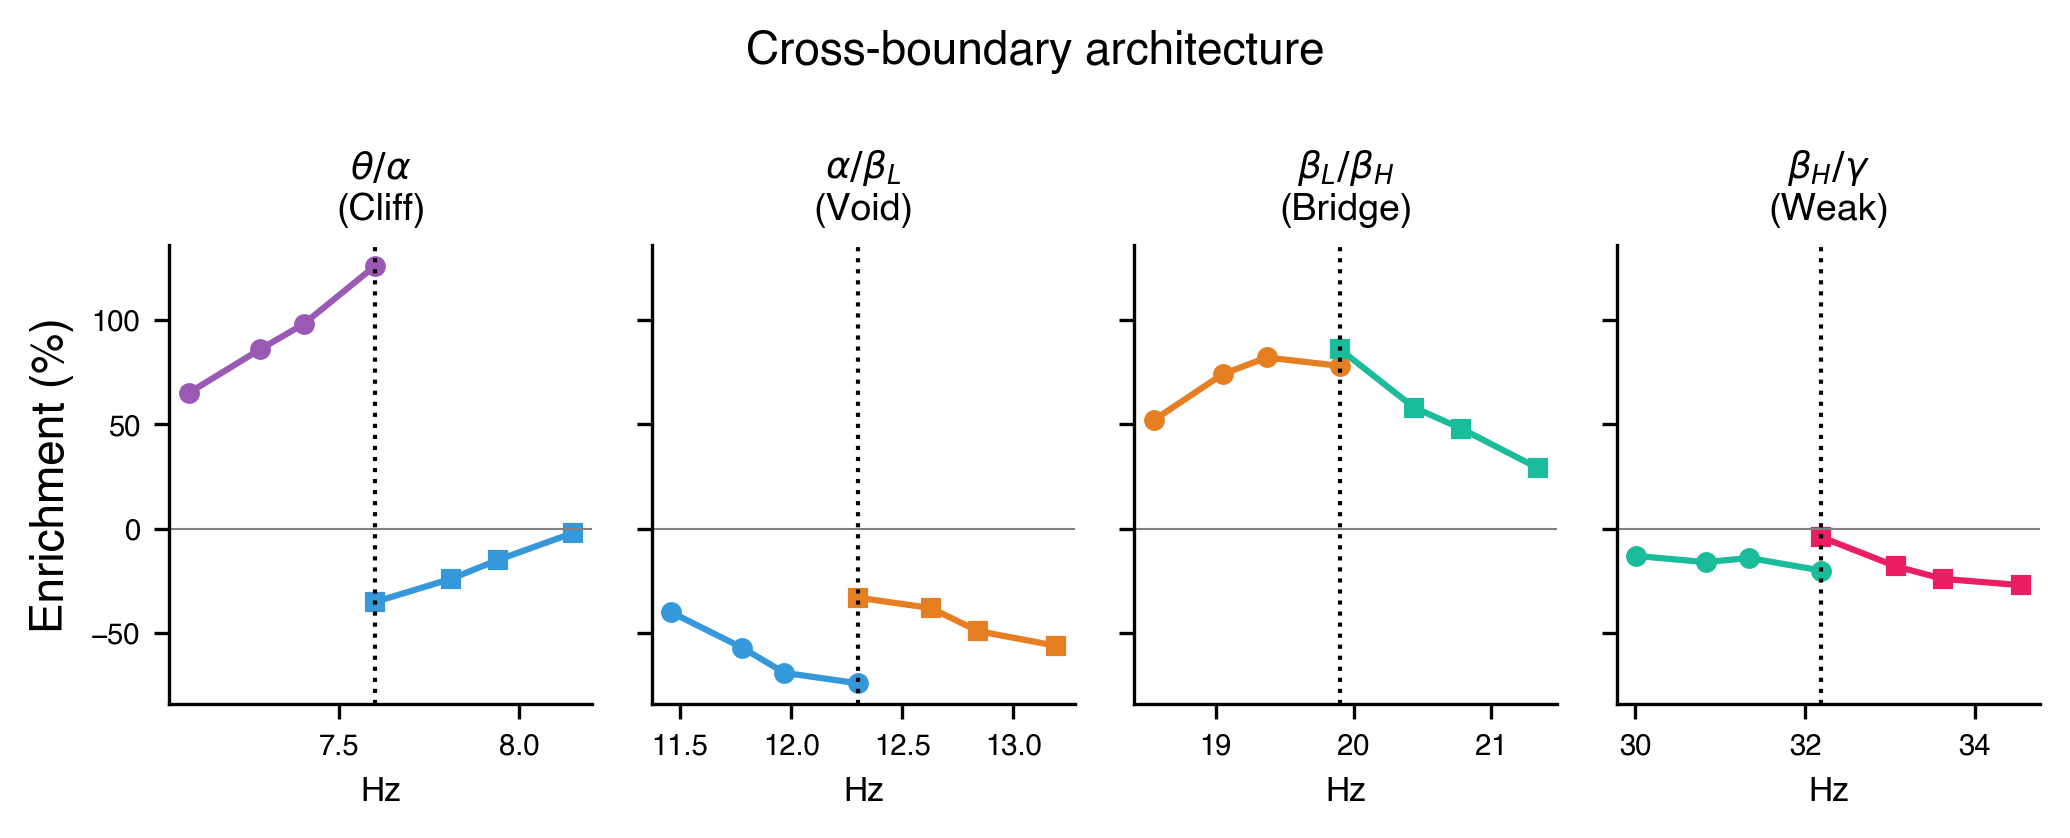
\includegraphics[width=\textwidth]{fig5_cross_boundary.png}
\caption{\textbf{Cross-boundary architecture.} Enrichment profiles near each of the four $\phisym$-lattice band boundaries, computed as 9-dataset mean Hz-corrected Voronoi enrichment ($N = 2{,}097$ subjects). Dotted vertical lines mark the boundary frequency. (Left to right:) The $\theta/\alpha$ boundary at 7.60~Hz is a cliff ($\Delta = -161$~pp); the $\alpha/\beta_L$ boundary at 12.30~Hz is a void (both sides depleted); the $\beta_L/\beta_H$ boundary at 19.90~Hz is a bridge (both sides enriched, $\Delta = +8$~pp); the $\beta_H/\gamma$ boundary at 32.19~Hz is weak. $\Delta$ is the signed difference in enrichment (above minus below boundary).}
\label{fig:cross_boundary}
\end{figure}

\subsubsection{Alpha is the Near-Exact Inverse of All Other Bands}
\label{sec:alpha-inverse}

The most structurally distinctive feature of the enrichment landscape is the systematic sign-inversion of alpha relative to all other bands. Across all 13 $\phisym$-lattice positions, the sign of alpha enrichment is opposite to theta, beta-low, and gamma, with a position-level correlation between the alpha and theta profiles of $r \approx -0.95$.

This anti-correlation organizes the octave into three functional zones. In the lower zone ($u = 0.00$--$0.38$), alpha is depleted ($-3\%$ to $-35\%$) while beta-high is enriched and theta, beta-low, and gamma are also largely depleted. In the mid zone ($u = 0.38$--$0.62$), alpha is strongly enriched ($+30\%$ to $+41\%$) while all other bands are depleted or null. In the upper zone ($u = 0.62$--$1.00$), alpha collapses strongly ($-5\%$ to $-73\%$) while theta ($+35\%$ to $+123\%$), beta-low ($+29\%$ to $+83\%$), and gamma ($+22\%$ to $+55\%$) rise in concert.

The extreme of the anti-correlation is at boundary\_hi (12.30 Hz): theta $+123\%$ versus alpha $-73\%$, a 196 pp gap between co-occurring peaks in the same $\phisym$-octave coordinate. The biophysical interpretation is that thalamocortical T-type Ca$^{2+}$ channel dynamics provide sufficient intrinsic resonance to pin alpha peaks to the mid-octave attractor and Noble$_1$ positions, actively opposing the upper-octave gradient that governs theta, beta-low, and gamma. Where alpha occupies the mid-octave, competing oscillatory modes are suppressed; where alpha vacates the upper octave, gradient-driven accumulation is unopposed.

\subsubsection{The $\approx$20 Hz Bridge}
\label{sec:bridge}

The $\beta_{\mathrm{L}}/\beta_{\mathrm{H}}$ boundary at 19.90 Hz ($= \fzero \times \phisym^2$) is the only band boundary in the $\phisym$-lattice that is enriched from both sides simultaneously. The beta-low ascending ramp peaks at inv\_noble$_6$ ($+87\%$, 19.37 Hz) before reaching boundary\_hi ($+83\%$, 19.90 Hz), while beta-high begins its descending ramp at its lower boundary ($+85\%$, 19.90 Hz), declining monotonically to boundary\_hi ($-18\%$, 32.19 Hz). The discontinuity across the 19.90 Hz boundary is only $+2$ pp---the smallest of any boundary and the only one consistent with continuity of spectral density.

This convergence from both sides constitutes a spectral attractor at $\approx$20 Hz that is independent of paradigm, age group, and recording system: all 9 datasets (4 adult, 5 pediatric HBN releases) show enrichment at the beta-low upper positions, and the bridge pattern is confirmed in resting-state datasets without any motor component.

The 19.90 Hz frequency satisfies the Fibonacci identity $\fzero + \fzero \times \phisym = \fzero \times \phisym^2$ (i.e., $7.60 + 12.30 = 19.90$~Hz). However, this identity is a mathematical tautology---it follows from $\phisym^2 = \phisym + 1$ and holds for any $\fzero$. It does not, by itself, explain why peaks converge at this frequency. The explanation must be biophysical: four mechanisms are known to peak at $\approx$20 Hz: (1) M-current KCNQ channel resonance ($\approx$50 ms time constant); (2) corticomuscular coherence (17--21 Hz during sustained contraction); (3) post-movement beta rebound ($\approx$19.4 Hz); and (4) the antikinetic frequency (20 Hz tACS reliably slows voluntary movement). These four are not necessarily independent---M-current resonance could be the common biophysical substrate underlying corticomuscular coherence and the antikinetic effect, in which case the apparent convergence of distinct mechanisms would reduce to a single channel-level time constant expressed across motor-system contexts. Whether the convergence of these processes at a frequency that happens to equal $\fzero \times \phisym^2$ reflects a deep organising principle or a coincidence of biophysical time constants is an open question that the present data cannot resolve. The bridge is an empirical finding; its interpretation remains speculative.


%------------------------------------------------------------------------------
\subsection{Part III: Spectral Differentiation as Biomarker}
\label{sec:biomarker}
%------------------------------------------------------------------------------

A biomarker must first be reliable before it can be meaningful. We therefore begin with temporal stability, then establish the developmental trajectory---the strongest and most replicated signal---before turning to cognitive associations, psychopathology, and informative nulls. The enrichment features derived from logarithmic $\phisym$-lattice coordinates carry systematic variance across lifespan development, cognitive performance, and psychopathology dimensions while remaining silent for personality, handedness, and metabolic variables.

\textbf{Gamma caveat.} Throughout this section, gamma-band results (32--52~Hz) should be interpreted with the scalp EEG contamination caveat described in Section~\ref{sec:two-regimes}: gamma had the weakest cross-dataset consistency (6/13 positions), the lowest test--retest reliability (ICC $= 0.250$), and is susceptible to electromyographic and microsaccade artifacts that standard preprocessing cannot fully remove. Gamma associations that replicate in artifact-controlled modalities (MEG, intracranial EEG) would be considerably more convincing than the scalp EEG results reported here.

\subsubsection{Five-Year Test--Retest Reliability of Spectral Differentiation (Dortmund, $N = 208$)}
\label{sec:testretest}

Intraclass correlation coefficients (ICC; two-way mixed, absolute agreement) were computed between session-1 and session-2 eyes-closed enrichment profiles in the longitudinal Dortmund subsample ($N = 208$; mean inter-session interval: approximately 5 years). Per-band median ICCs are reported in Table~\ref{tab:icc}.

Beta-low enrichment was the most temporally stable band (median ICC $= 0.604$), followed by beta-high ($0.507$), alpha ($0.454$), theta ($0.382$), and gamma ($0.250$, the lowest); the cross-band median was $0.421$. At the individual-feature level, beta-low \textit{ushape} achieved ICC $= 0.746$, the highest five-year stability in the entire feature set.

Group-level profile stability was evaluated by correlating the 12-position enrichment vectors between sessions for each band. All five bands exceeded $r = 0.96$: beta-low $r = 0.988$, beta-high $r = 0.987$, theta $r = 0.983$, alpha $r = 0.977$, gamma $r = 0.964$. The pattern of eyes-closed to eyes-open change (EC$\to$EO delta vectors) was itself stable across the five-year interval ($r = 0.875$--$0.990$). Age did not predict five-year change in any enrichment feature (0 FDR across 90 tests).

\begin{table}[htbp]
\centering
\caption{Five-year test--retest ICCs for $\phisym$-lattice enrichment, Dortmund longitudinal ($N = 208$). Earlier extraction pipelines with restrictive peak caps produced negative ICCs ($-0.25$ to $-0.36$); the corrected pipeline yields strongly positive values.}
\label{tab:icc}
\begin{tabular}{lrr}
\toprule
\textbf{Band} & \textbf{Median ICC} & \textbf{Most Stable Feature (ICC)} \\
\midrule
Beta-low  & $0.604$ & beta\_low\_ushape ($0.746$) \\
Beta-high & $0.507$ & -- \\
Alpha     & $0.454$ & -- \\
Theta     & $0.382$ & -- \\
Gamma     & $0.250$ & -- \\
\midrule
\textbf{Overall} & $\mathbf{0.421}$ & \\
\bottomrule
\end{tabular}
\end{table}

\begin{figure}[htbp]
\centering
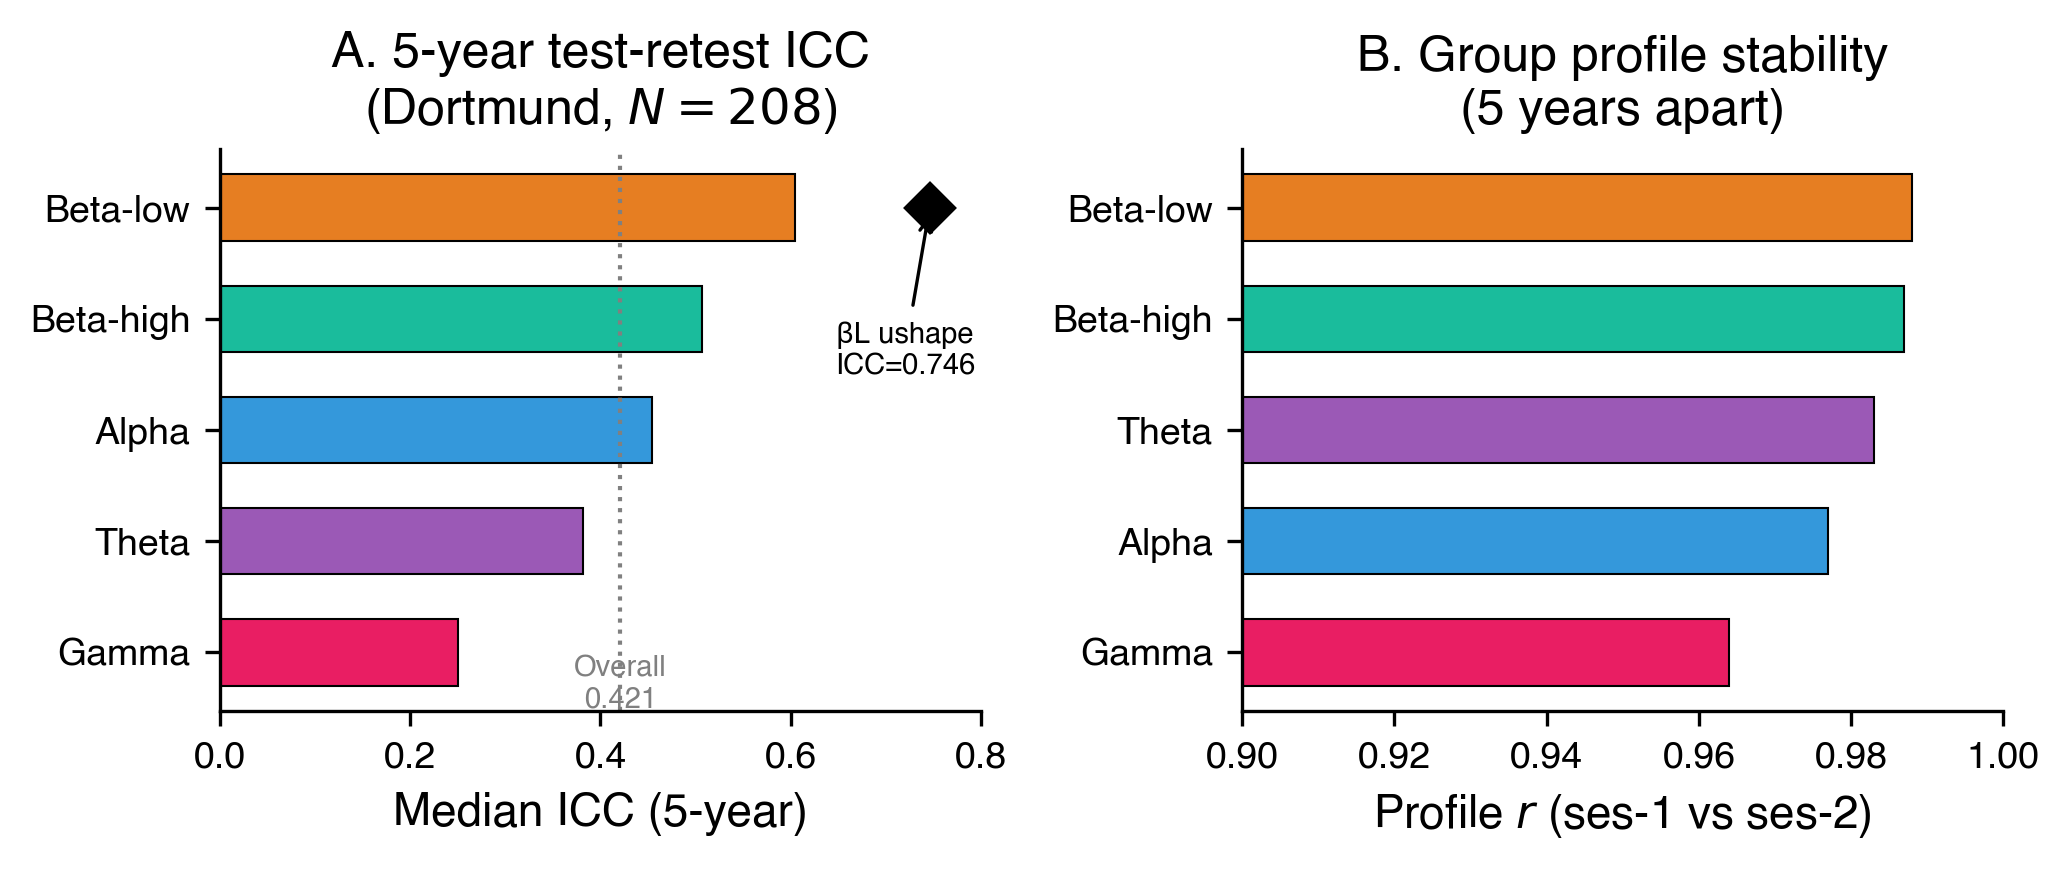
\includegraphics[width=\textwidth]{fig8_reliability.png}
\caption{\textbf{Five-year test--retest reliability.} (A)~Median intraclass correlation coefficient (ICC; two-way mixed, absolute agreement) per band across $\sim$5 years (Dortmund longitudinal subsample, $N = 208$ subjects, eyes-closed). Beta-low is the most stable band (median ICC $= 0.604$); the single most stable feature is beta-low ushape (ICC $= 0.746$, diamond). Gray dotted line: cross-band median ($0.421$). (B)~Group enrichment profile correlations (Pearson $r$) between session-1 and session-2 12-position enrichment vectors. All bands exceed $r = 0.96$, indicating that the population-level enrichment pattern is virtually identical 5 years apart.}
\label{fig:reliability}
\end{figure}

\subsubsection{Developmental Trajectory (HBN, $N = 927$, Ages 5--21)}
\label{sec:development}

All 90 enrichment features were correlated with age (continuous, in years) in the HBN pediatric dataset. Sixty tests survived FDR correction ($q < 0.05$ across 90 tests).

The strongest developmental feature was alpha \textit{inv\_noble$_4$} ($\rho = +0.354$, $p_\text{FDR} < 0.0001$): the upper flank of the alpha mountain broadens progressively throughout development, extending enrichment toward higher-frequency positions. This asymmetric broadening is corroborated by alpha \textit{asymmetry} ($\rho = +0.351$) and alpha \textit{ramp\_depth} ($\rho = +0.328$). Simultaneously, the beta-low center clears (noble$_3$: $\rho = -0.194$, $p_\text{FDR} < 0.0001$) and gamma ramp sharpens modestly (noble$_3$: $\rho = -0.207$).

Cross-release stability was assessed by correlating developmental effect vectors across the five independent HBN data releases (R1--R6, $N = 136$--322 per release). The mean inter-release Pearson correlation was $r = 0.787$. Alpha showed 13/13 position agreement on the sign of enrichment across release $\times$ position cells.

A caveat is warranted: IAF correlates with age substantially more strongly in HBN ($\rho = +0.362$, $p < 10^{-29}$, $N = 915$) than in the adult LEMON sample where IAF-partialing was performed. This IAF--age effect is comparable in magnitude to the top enrichment--age correlation reported above ($\rho = +0.354$ for alpha inv\_noble$_4$), indicating that a substantial fraction of the developmental enrichment signal may be mediated through IAF maturation rather than genuine within-band reorganization. IAF-partialed developmental correlations are not presented for HBN because the strong IAF--age collinearity ($\rho = 0.362$) makes partialing unstable: removing IAF variance necessarily removes most age variance and vice versa, yielding uninterpretable partial correlations. In the adult LEMON sample, IAF--age collinearity is weaker, permitting clean separation. Features that are most IAF-sensitive in the LEMON partialing analysis (beta-low ramp metrics, Section~\ref{sec:cognitive}) should be interpreted with proportionally greater caution in the developmental context than IAF-insensitive features (gamma ramp, theta boundary convergence).

\subsubsection{Aging Trajectory (Dortmund, $N = 608$, Ages 20--70)}
\label{sec:aging}

In the adult Dortmund sample spanning ages 20--70, 41 tests survived FDR correction. The direction of every major age effect was opposite to the developmental direction in HBN. During development, alpha \textit{inv\_noble$_3$} increases ($\rho = +0.301$); during adult aging it decreases ($\rho = -0.276$, $p_\text{FDR} < 0.001$)---the alpha mountain progressively narrows. During development, the beta-low interior clears; during adult aging, the beta-low attractor fills in ($\rho = +0.311$, $p_\text{FDR} < 0.001$)---the ascending ramp flattens.

\subsubsection{Inverted-U Lifespan Trajectory}
\label{sec:lifespan}

Combining the pediatric (HBN) and adult (Dortmund) datasets reveals a systematic inverted-U trajectory of spectral differentiation across the human lifespan. Of 31 enrichment features that reached FDR significance in at least two of the three datasets (HBN, Dortmund, LEMON), 28 showed opposite signs in the developmental versus aging comparisons ($28/31 = 90\%$). Under development, enrichment profiles become more differentiated---peaks concentrate more tightly at canonical positions; under aging, they progressively de-differentiate.

To estimate the vertex of this trajectory, we fit quadratic models to the combined HBN + Dortmund age range (5--70 years, $N = 1{,}465$--$1{,}535$ depending on metric). The quadratic model was decisively superior to linear for the three strongest features ($\Delta$BIC $> 45$). The vertex---the age at which spectral differentiation is maximal---fell consistently at \textbf{33--35 years}: alpha asymmetry 35.0 years (95\% bootstrap CI [33.5, 36.6], $R^2 = 0.093$), alpha inv\_noble$_4$ 35.2 years ([33.3, 37.5]), and beta-low ushape 33.2 years ([31.2, 35.2]). This is later than the ~20-year estimate suggested by the dataset boundary alone, and coincides more closely with the completion of cortical myelination (which continues into the early 30s) and peak cognitive performance in fluid reasoning tasks. However, the vertex estimate should be interpreted with caution: it falls near the splice point of the two contributing datasets (HBN ends at 21, Dortmund begins at 20), which have different recording systems, countries, and demographic compositions. Quadratic fits to Dortmund alone (ages 20--70, $N = 483$--507) do not support an inverted-U within that cohort: $\Delta$BIC favors linear over quadratic for all three features, and the Dortmund trajectory is monotonically declining throughout the adult range. The inverted-U is therefore driven entirely by the cross-cohort splice between developmental increase (HBN) and adult decline (Dortmund), not by a within-cohort turning point. The bootstrap CIs on the combined vertex quantify sampling uncertainty but do not address this between-dataset confound. Longitudinal data spanning childhood through middle age within a single cohort would be needed to confirm whether 33--35 years is the genuine vertex or an artifact of the cross-sectional splice.

\begin{figure}[htbp]
\centering
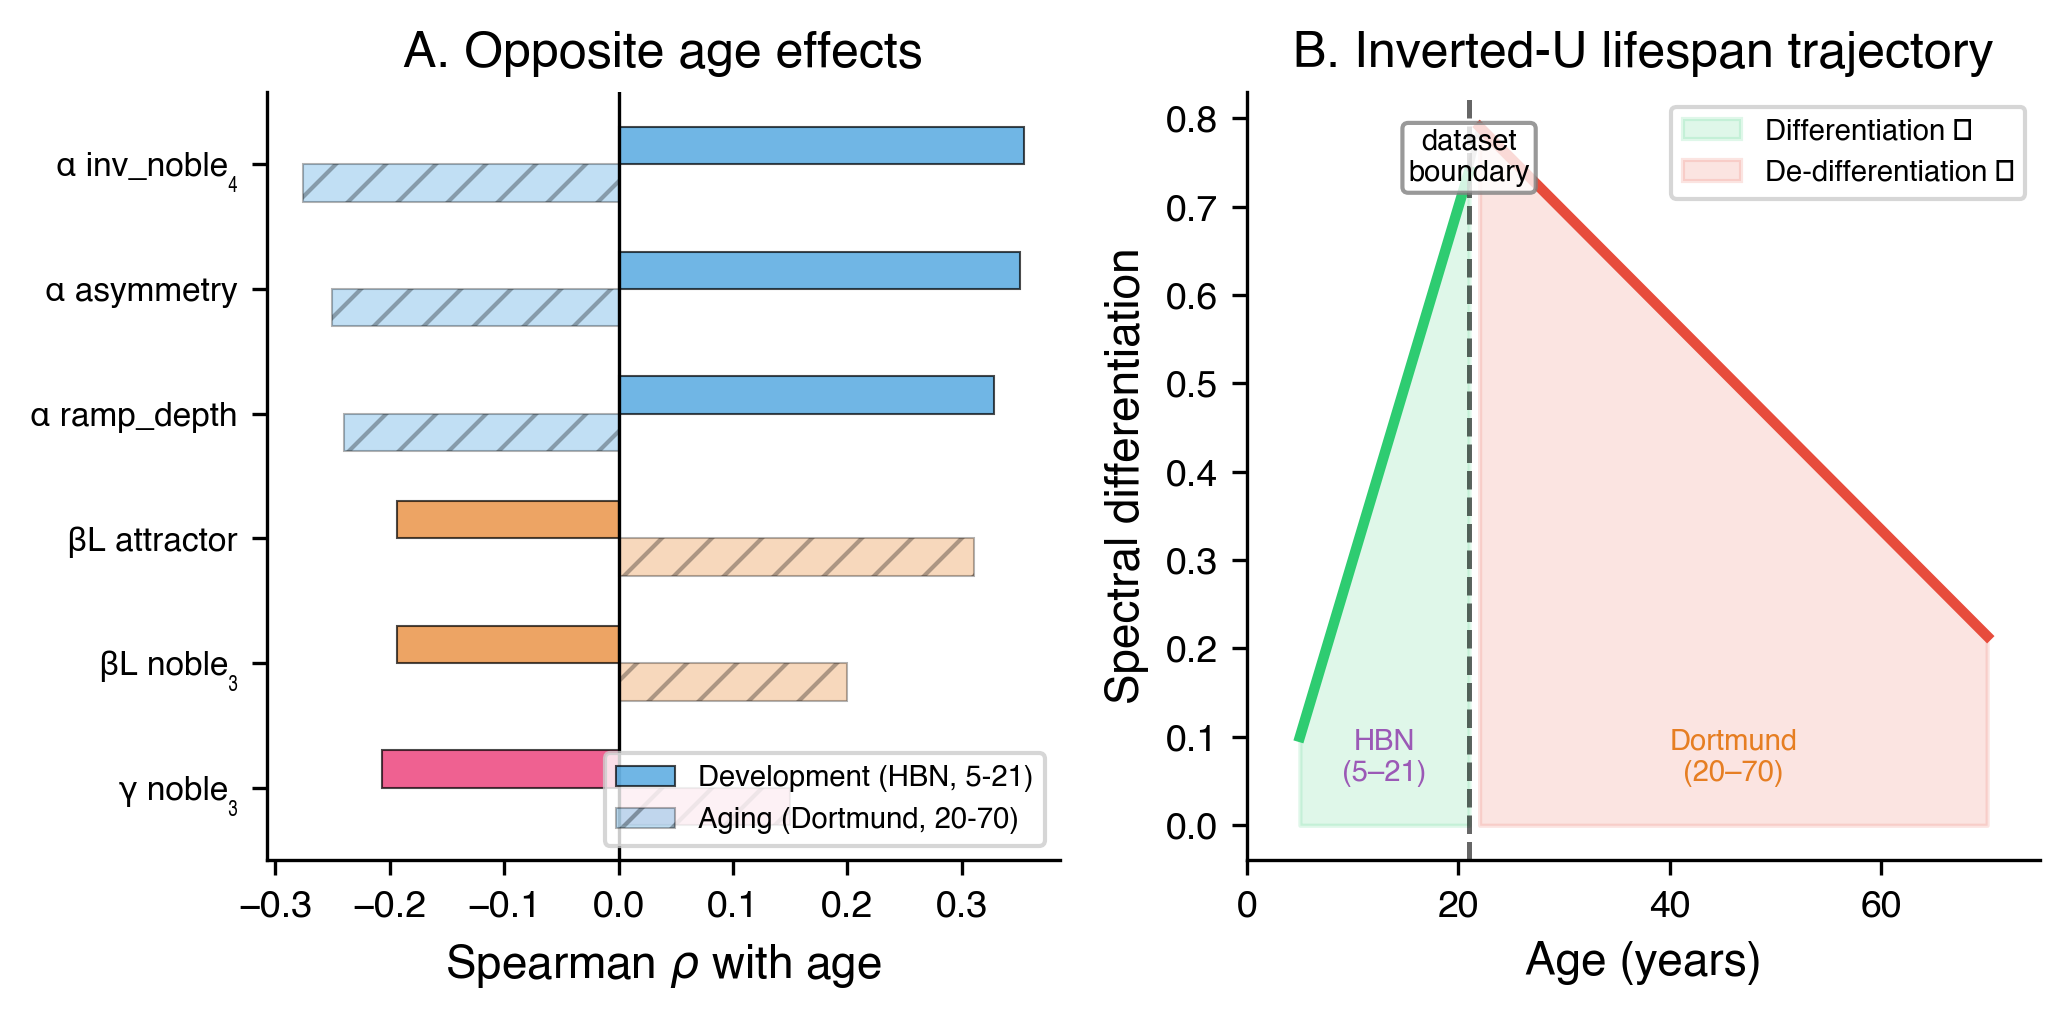
\includegraphics[width=\textwidth]{fig7_lifespan.png}
\caption{\textbf{Inverted-U lifespan trajectory of spectral differentiation.} (A)~Spearman rank correlations ($\rho$) with age for key enrichment features in the developmental (HBN, $N = 927$, ages 5--21, solid bars) and aging (Dortmund, $N = 608$, ages 20--70, hatched bars) datasets. FDR correction: Benjamini--Hochberg $q < 0.05$ across 90 tests per dataset; 60 survivors in HBN, 41 in Dortmund. Every major feature shows opposite signs: differentiation increases during development and decreases during aging. (B)~Schematic inverted-U trajectory. Quadratic fits (ordinary least squares) to the combined 5--70-year age range ($N = 1{,}465$--$1{,}535$) place the vertex at $\sim$33--35 years (95\% bootstrap CIs: alpha asymmetry [33.5, 36.6]; see text), coinciding with the completion of cortical myelination.}
\label{fig:lifespan}
\end{figure}

\subsubsection{Cognitive Correlates (LEMON, $N = 203$)}
\label{sec:cognitive}

Spearman correlations were computed between all 90 enrichment features and eight neuropsychological scores from the LEMON battery (eyes-closed condition) and corrected for multiple comparisons using the Benjamini--Hochberg false-discovery-rate (FDR) procedure at $q < 0.05$ across $720$ simultaneous tests ($90$ features $\times$ $8$ scores). Thirty-one tests survived FDR correction, spanning four cognitive domains and four frequency bands (Table~\ref{tab:cog_top}).

The strongest association was between beta-low \textit{center\_depletion} and logical reasoning (LPS): $\rho = -0.273$, $p_\text{FDR} = 0.024$. The negative sign indicates that individuals whose beta-low band is more deeply cleared in its interior---a steeper ascending ramp toward the $\phisym$-lattice upper boundary---achieve higher reasoning scores. The second-ranked association linked theta \textit{ushape} with the TAP incompatibility reaction-time score ($\rho = +0.267$, $p_\text{FDR} = 0.024$): greater theta spectral differentiation corresponds to faster executive conflict resolution. Upper-gamma enrichment at the inv\_noble$_4$ position predicted verbal fluency on the Regensburg Word Test (RWT; $\rho = +0.260$, $p_\text{FDR} = 0.024$), and alpha \textit{inv\_noble$_6$} predicted Trail-Making Test performance ($\rho = -0.253$, $p_\text{FDR} = 0.024$).

To test whether the cognitive associations survive replication across vigilance states, the same analysis was repeated on the eyes-open (EO) condition ($N = 202$; the slight difference from the EC sample of 203 reflects subjects whose EO recordings passed quality thresholds while their EC recordings did not, or vice versa). Twenty-five tests survived FDR correction under EO, encompassing the same four cognitive domains and the same three bands (beta-low, theta, gamma); the top effect was \textit{beta\_low\_mountain} $\times$ LPS ($\rho = -0.312$, $p_\text{FDR} = 0.004$). The cognitive signal is therefore not specific to the eyes-closed state.

\paragraph{Age-partialed analysis.}
The LPS correlation attenuated from $\rho = -0.273$ to $\rho_\text{partial} = -0.153$ ($p = 0.030$) after partialing out age, a 44\% reduction. The effect survives age control, indicating that approximately half the association is genuine cognitive variance and approximately half is mediated through age-related sharpening of spectral differentiation (Section~\ref{sec:development}).

\paragraph{IAF-partialed analysis.}
The age-partialing analysis leaves open whether the cognitive signal is driven by individual differences in $\fzero$ placement rather than genuine within-band organization---since subjects whose IAF deviates from the population $\fzero = 7.60$~Hz have systematically misaligned boundaries that could masquerade as low differentiation. To test this, we computed each subject's IAF as the power-weighted centroid of specparam-detected alpha-band peaks (mean $= 9.83 \pm 0.67$~Hz, range 8.27--11.61~Hz) and repeated the cognitive correlations partialing out IAF. Among 46 features with raw $|\rho| > 0.20$, IAF-partialing attenuated mean effect size by 23\% (from 0.240 to 0.185), with 31/46 surviving $p < 0.05$. By comparison, age-partialing produced 47\% attenuation, and combined age+IAF partialing produced 51\%---meaning IAF adds only 4 percentage points of attenuation beyond age alone, reflecting the substantial collinearity between IAF and age across LEMON's 20--77-year range. The attenuation was band-specific: gamma features were nearly unaffected (gamma\_inv\_noble$_4$ $\times$ LPS: $\rho = +0.287 \to +0.273$), consistent with IAF having no direct influence on gamma-band boundaries, while beta-low features showed larger reductions (center\_depletion $\times$ LPS: $-0.248 \to -0.127$), consistent with the alpha mountain's upper flank partly determining beta-low ramp position. Spectral differentiation captures within-band organizational variance that is largely independent of where an individual's alpha peak sits.

\paragraph{Personality null.}
The same 90 features were correlated with all 133 personality and emotion subscales available in the LEMON battery (11,970 tests). Zero tests survived FDR correction. Spectral differentiation predicts cognitive performance but is psychometrically silent for personality traits.

\begin{table}[htbp]
\centering
\caption{Top FDR-significant enrichment $\times$ cognition correlations, LEMON eyes-closed ($N = 203$, $q < 0.05$ FDR across 720 tests). LPS = logical reasoning; TAP = incompatibility reaction time; RWT = verbal fluency; TMT = Trail Making Test.}
\label{tab:cog_top}
\begin{threeparttable}
\begin{tabular}{llrr}
\toprule
\textbf{Test} & \textbf{Feature} & $\boldsymbol{\rho}$ & $\boldsymbol{p_\text{FDR}}$ \\
\midrule
LPS   & beta\_low\_center\_depletion  & $-0.273$ & $0.024$ \\
TAP   & theta\_ushape                  & $+0.267$ & $0.024$ \\
TAP   & theta\_boundary                & $+0.263$ & $0.024$ \\
TAP   & theta\_mountain                & $-0.260$ & $0.024$ \\
RWT   & gamma\_inv\_noble\_4           & $+0.260$ & $0.024$ \\
RWT   & gamma\_ramp\_depth             & $+0.256$ & $0.024$ \\
TMT   & alpha\_inv\_noble\_6           & $-0.253$ & $0.024$ \\
LPS   & beta\_low\_mountain            & $-0.250$ & $0.024$ \\
LPS   & beta\_low\_ushape              & $+0.249$ & $0.024$ \\
LPS   & beta\_low\_attractor           & $-0.245$ & $0.024$ \\
LPS   & gamma\_inv\_noble\_4           & $+0.243$ & $0.025$ \\
LPS   & beta\_low\_boundary            & $+0.240$ & $0.026$ \\
\bottomrule
\end{tabular}
\begin{tablenotes}
  \small
  \item Age-partialed top correlation: $\rho_\text{partial} = -0.153$, $p = 0.030$.
        IAF-partialed: 23\% mean attenuation; 31/46 features with $|\rho| > 0.20$ survive $p < 0.05$.
        EO replication: 25 FDR survivors with peak $\rho = -0.312$.
\end{tablenotes}
\end{threeparttable}
\end{table}

\begin{figure}[htbp]
\centering
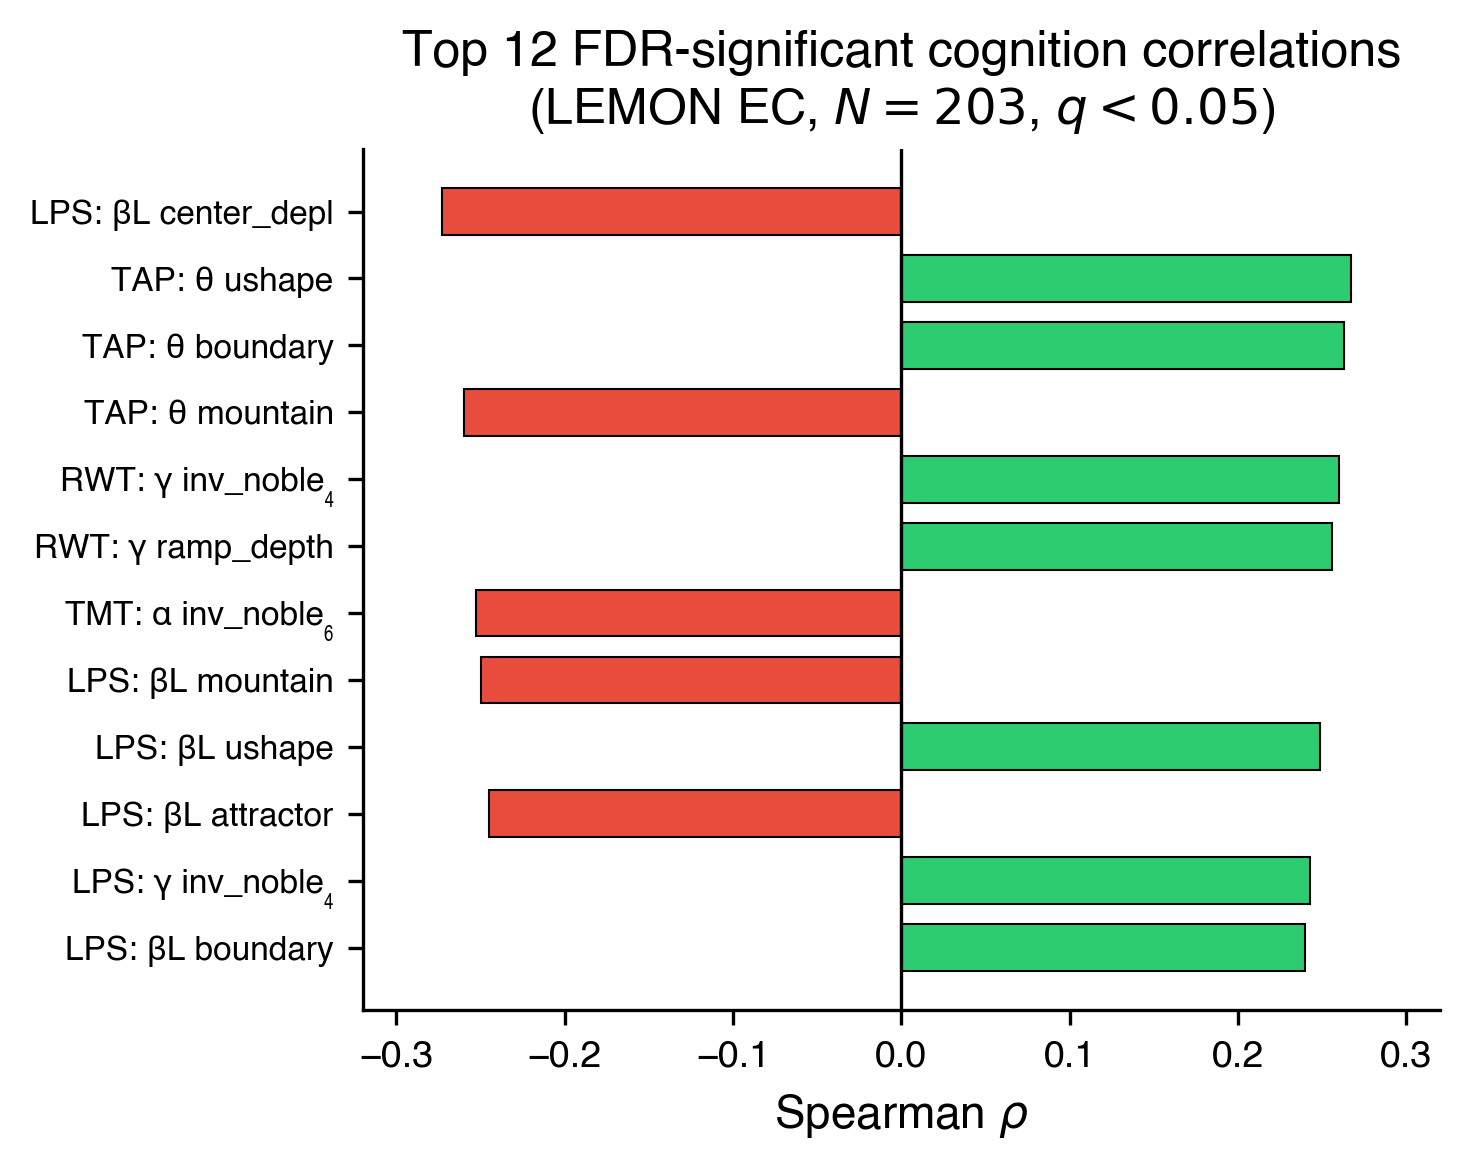
\includegraphics[width=0.65\textwidth]{fig6_cognitive.png}
\caption{\textbf{Top 12 FDR-significant cognition correlations.} Spearman rank correlations ($\rho$) between enrichment features and cognitive test scores (LEMON eyes-closed, $N = 203$ subjects, Benjamini--Hochberg FDR $q < 0.05$ across 720 simultaneous tests). Green bars: positive correlations (higher enrichment = better performance); red bars: negative correlations (steeper ramp = better performance). Error bars are not shown as these are rank correlations; exact $p_\text{FDR}$ values are reported in Table~\ref{tab:cog_top}. Four cognitive domains (LPS reasoning, TAP executive control, RWT verbal fluency, TMT trail-making) and four frequency bands (beta-low, theta, gamma, alpha) are represented.}
\label{fig:cognitive}
\end{figure}

\subsubsection{Psychopathology (HBN, $N = 906$)}
\label{sec:psychopathology}

Enrichment features were correlated with dimensional psychopathology scores (externalizing, internalizing, p-factor, and attention subscales) derived from the Child Behavior Checklist (CBCL).

\textbf{Externalizing.} Eighteen features survived FDR correction, all in the direction of \textit{flatter} enrichment profiles: gamma \textit{inv\_noble$_4$} ($\rho = -0.159$) and beta-low \textit{inv\_noble$_1$} ($\rho = +0.127$) represent reduced spectral differentiation across multiple bands. Higher externalizing scores are associated with less concentrated, less differentiated spectral architecture.

\textbf{Internalizing.} Seven features survived FDR correction. Critically, the direction was dissociable from externalizing: internalizing was associated with \textit{more} upper-alpha enrichment (alpha\_inv\_noble$_4$: $\rho = +0.126$), the opposite of the externalizing pattern in that band. Steiger's $z$-tests for dependent correlations confirmed that the externalizing and internalizing associations were significantly different in direction for all five features tested (all $z > 2.9$, all $p < 0.004$; externalizing--internalizing correlation $r = -0.22$, $N = 906$). The dissociation is formally significant, not merely descriptive.

\textbf{General and attentional factors.} The p-factor and attention subscales each yielded zero FDR survivors, confirming that enrichment-psychopathology associations are specific to the externalizing--internalizing dimension and are not driven by general symptom severity.

\subsubsection{Informative Nulls}
\label{sec:nulls}

Every falsification criterion was satisfied. Personality and emotion subscales: 0/11,970 FDR (LEMON). Medical and metabolic markers: 0 FDR across approximately 2,500 tests (LEMON). Handedness: 0 FDR (HBN continuous and dichotomized; Dortmund). Sex $\times$ age interaction: 0 FDR (HBN and Dortmund). State $\times$ age interaction: 0 FDR (LEMON and Dortmund).

The contrast between 31 cognitive FDR survivors and zero personality FDR survivors, across the same 90 features and the same subjects, establishes that enrichment features are selectively predictive of cognitive performance, not globally correlated with individual-differences variables.

\subsubsection{Cross-Band Coupling}
\label{sec:coupling}

All pairwise Spearman correlations among the 90 enrichment features were computed within each dataset. In HBN ($N = 927$), 93 cross-band feature pairs survived FDR correction. The dominant coupling was between alpha and beta-low: alpha \textit{noble$_1$} $\times$ beta-low \textit{ushape} reached $\rho = +0.412$ ($p_\text{FDR} < 0.0001$) in HBN and replicated at $\rho = +0.344$ ($p_\text{FDR} < 0.001$) in Dortmund. Individuals with taller, more concentrated alpha mountains simultaneously exhibit deeper, more differentiated beta-low ascending ramps. This alpha--beta-low coupling is interior-only (involving no boundary positions), ruling out boundary-artifact cross-band coupling reported previously \parencite{lacy2026frontiers}. The coupling product was individually stable within-session ($r = +0.393$, $p < 10^{-22}$). By contrast, beta-low and gamma features were essentially uncoupled ($\rho \approx 0$).

\subsubsection{Cross-Release Consistency (HBN, Five Independent Releases)}
\label{sec:crossrelease}

Enrichment profiles were computed independently for each HBN release ($N = 136$--322 per release). Alpha showed 13/13 position-$\times$-release agreements on enrichment sign, and the inv\_noble$_1$ position had a standard deviation of only 1.0 percentage points across releases---the most reproducible cross-sample finding. The cross-release developmental effect vector had a mean inter-release Pearson correlation of $r = 0.787$, indicating that the developmental trajectory is stable across independent acquisition batches.

\subsubsection{State Sensitivity and State Invariance}
\label{sec:state}

Theta was the most state-sensitive band: the boundary\_hi position enrichment was $+128\%$ (EC) versus $+48\%$ (EO) in Dortmund, a $\Delta$ of 80 pp. This theta state-sensitivity reflects $\fzero$ convergence: under eyes-closed conditions, theta peaks concentrate strongly toward 7.60 Hz. Beta-low ramp contrast attenuates under EO (shape preserved, magnitude reduced). Alpha mountain sharpens under EC (attractor: $+41\%$ EC versus $+36\%$ EO).

Gamma enrichment was state-invariant: the maximum EC--EO difference at any gamma position was 14 pp. State sensitivity was age-independent: zero FDR survivors when EC--EO delta magnitude was regressed on age in either LEMON or Dortmund (90 tests each). The selective responsiveness of theta and the invariance of gamma are properties of the frequency architecture itself, not epiphenomena of age-related vigilance differences.

%------------------------------------------------------------------------------
\subsection{Part IV: Method-Independence Check}
\label{sec:irasa}
%------------------------------------------------------------------------------

All preceding results use FOOOF/specparam for aperiodic-periodic separation. To test whether the enrichment landscape depends on this specific parametric approach, we replicated the full extraction and analysis pipeline using IRASA (Irregular Resampling Auto-Spectral Analysis), a non-parametric method that isolates the aperiodic component through resampling at irrational factors rather than fitting a parametric $1/f$ model \parencite{wen2016irasa}. Band-adaptive resampling factors were selected following \textcite{gerster2022irasa} to avoid highpass edge and noise floor contamination; all downstream analyses (band assignment, Voronoi enrichment, power filtering, per-subject metrics) were identical.

Three results establish selective method-independence. First, the beta-high descending ramp achieved 12/13 mean-level sign agreement with FOOOF and 13/13 cross-dataset consistency under IRASA (versus 5/13 under FOOOF), with a steeper gradient (192 versus 113 percentage points). Beta-high is more robust under IRASA than under FOOOF. Second, the core cognitive association replicated: beta-low ramp $\times$ LPS reasoning reached $\rho = -0.294$ under IRASA ($p_\text{FDR} < 0.02$), comparable to FOOOF's $\rho = -0.278$ ($p_\text{FDR} < 0.02$). IRASA produced 8 cognitive FDR survivors overall (versus 31 under FOOOF). A peak-yield subsample test established that this gap is largely attributable to IRASA's reduced per-subject peak yield rather than to fundamentally different enrichment patterns: IRASA yields only 46\% as many theta peaks and 63--65\% as many alpha and beta-low peaks per subject as FOOOF (though beta-high and gamma are closer to parity at 71--82\%). When FOOOF peaks were randomly subsampled to match IRASA's per-band yield ratios ($N = 200$ iterations), the mean FDR survivor count dropped by approximately 40\%, substantially narrowing the gap; 30\% of subsample iterations produced $\leq$2 FDR survivors, comparable to the IRASA result. The FOOOF--IRASA cognitive gap is thus primarily a statistical power artefact of lower peak yield in the bands that carry the strongest cognitive signal, rather than evidence that FOOOF's enrichment patterns are parametric artefacts. Third, developmental trajectories were equally robust: both methods yielded 68/90 FDR-significant age correlations in HBN, dominated by the same alpha features, with IRASA producing larger top effect sizes ($\rho$ up to $0.417$ versus $0.362$).

Not all bands replicated. Theta enrichment profiles were substantially inverted between methods (5/13 sign agreement)---an expected failure mode when IRASA's evaluated frequency range extends below the highpass filter edge \parencite{gerster2022irasa}. Gamma remained inconsistent under both methods. The enrichment landscape is selectively method-independent: the strongest structural, cognitive, and developmental findings survive fundamentally different aperiodic decomposition approaches; low-frequency and high-frequency band profiles remain method-sensitive.


%==============================================================================
% DISCUSSION
%==============================================================================
\section{Discussion}

This study makes two contributions of different character. The first is a \emph{coordinate system}---a log-frequency partition of the EEG spectrum whose boundary positions are empirically optimised, whose scaling ratio is identified by subject-level bootstrap, and whose validity is tested against alternatives with formal model comparison. The second is a \emph{biomarker}---spectral differentiation, a class of within-band individual-differences measures that emerges only when the coordinate system is well-calibrated. The coordinate system is methodological infrastructure; the biomarker is the empirical payload.

These contributions rest on three levels of evidence that should not be conflated. \textbf{Directly observed:} log-frequency geometry, five genuine density troughs, within-band enrichment shapes, age and cognitive and psychopathology associations, test--retest reliability. \textbf{Inferential interpretations:} the alpha mountain as thalamocortical resonance, the $\sim$20~Hz bridge as convergent biophysical time constants, the developmental tuning account of the inverted-U. \textbf{Mechanistic hypotheses to test:} PV+ interneuron maturation as the driver of $\alpha$/$\beta$ trough deepening, GABAergic manipulation predictions, thalamocortical pathology sensitivity, source-localised regional specificity. The IRASA replication provides the sharpest calibration of what is robust: the strongest enrichment structure, the core cognitive association (beta-low differentiation $\times$ reasoning), and the developmental trajectory all survive a fundamentally different aperiodic decomposition method; the broader cognitive map and theta/gamma fine structure do not. The sections below treat each contribution in turn, and Section~3.7 formalises the distinction between robust and provisional claims.

\subsection{Logarithmic Frequency Scaling and the Global Scaling Constant}

The central empirical question of this paper---whether EEG band boundaries follow a logarithmic or linear progression---is answered decisively by the data. Across every dataset and every boundary estimation method, the log-linear model outperforms its arithmetic counterpart by $\Delta$BIC $> 50$, a difference conventionally interpreted as overwhelming evidence. The brain does not divide its spectral territory into equal-bandwidth slices; it divides it into equal-ratio slices, consistent with decades of informal practice in the field and with the theoretical arguments advanced by \textcite{penttonen2003natural}, \textcite{pletzer2010golden}, and \textcite{buzsaki2004neuronal}.

A BIC model comparison across seven candidate ratios initially suggested that the specific scaling constant was ambiguous: $\phisym$, $\sqrt{2}$, and $e - 1$ were mutually indistinguishable ($\Delta$BIC $< 2$). The subject-level bootstrap (Section~\ref{sec:bootstrap}) resolves this ambiguity by shifting the estimand from individual boundary ratios (which are heterogeneous, ranging from 1.36 to 1.89) to the \emph{global} geometric mean---the multiplicative constant that best summarises the five-trough sequence as a whole. At this level, the 95\% CI is [1.609, 1.623], containing $\phisym = 1.618$ while excluding $\sqrt{2}$, $e - 1$, and all other named candidates (all $p < 0.0001$).

This is a strong result but requires careful scoping. It establishes $\phisym$ as the uniquely supported \emph{global coordinate constant} among the candidate theories tested---not as the only possible real number near 1.618. The CI excludes the named competitors but does not exclude, say, 1.615 or 1.620. The claim is: \textbf{of the mathematical constants proposed in the frequency-scaling literature ($e$, $\phisym$, $e-1$, $\sqrt{2}$, $\sqrt{3}$, 2, $2^{1/3}$), only $\phisym$ is compatible with the subject-level evidence.} It does not follow that every adjacent boundary pair is individually $\phisym$-spaced; the local ratios remain irregular and hierarchical. The hierarchy has a coarse scale (three major troughs with ratio $\approx \phisym^2 \approx 2.6$) and a fine scale (five troughs with global ratio $\approx \phisym$), and both are real.

One candidate is excluded with particular force. The natural base $e \approx 2.718$ proposed by \textcite{penttonen2003natural} as the fundamental scaling constant implies inter-band ratios far wider than observed ($\Delta$BIC $> 11$ relative to $\phisym$; excluded by the bootstrap at $p < 0.0001$). The original observation appears to have been based on a selected subset of known band centres rather than systematic peak detection.

\paragraph{Reconciliation with Ursachi (2026).}
\textcite{ursachi2026boundaries} reported that three independent data-driven boundary-detection methods converge on a ratio of $e - 1 \approx 1.718$ rather than $\phisym \approx 1.618$, using $N = 244$ subjects. Our pooled BIC analysis favors $\phisym$ ($-24.74$ vs.\ $-23.06$ for $e - 1$), but this difference is not decisive ($\Delta$BIC $= 1.68$). The two studies' point estimates ($\phisym = 1.618$ vs.\ $e - 1 = 1.718$) differ by only 6\%---well within the variability of per-dataset ratio estimates (log-SD $= 0.26$). Our subject-level bootstrap excludes $e - 1$ at $p < 0.0001$, which is a genuine disagreement with Ursachi's point estimate rather than a methodological nuance. The most likely explanation is that Ursachi's methods detect only the three deepest troughs (geometric mean ratio $\approx 2.5$, biased toward higher values), while our larger pooled sample resolves the two shallower boundaries that bring the global ratio to $\phisym$. Ursachi's power-analysis finding that $N < 30$ systematically favors $\phisym$ does not apply here (our per-dataset $N$s range from 109 to 777), but it appropriately cautions against over-interpreting the specific constant in any single sample. The substantive agreement between the two studies is more important than the constant: both find logarithmic scaling with a ratio in the 1.6--1.7 range, both exclude $e$ and linear spacing, and both confirm that band boundaries are empirical realities rather than analytical conventions.

\subsection{The Enrichment Landscape as an Empirical Contribution}

The within-band enrichment profiles described in Part~II constitute a novel empirical characterization of spectral peak organization that stands independently of the biomarker analyses. Three findings merit emphasis.

First, the two-regime structure---alpha mountain versus ascending ramp---reveals that the canonical frequency bands are not organized by a single mechanism. Alpha's enrichment profile is the precise inverse of all other bands ($r \approx -0.95$ with theta), creating a three-zone octave structure in which the mid-octave belongs exclusively to alpha while the upper octave belongs to everything else. This sign-inversion is consistent with the known thalamocortical origin of the alpha rhythm but has not, to our knowledge, been documented quantitatively at this resolution across multiple datasets. It implies that aggregate enrichment measures---which average across bands---systematically cancel the alpha mountain against the ramps, producing misleadingly small effects. The per-band analysis is not merely more informative; it is necessary.

Second, the cross-boundary typology (cliff, void, bridge, weak) provides a new vocabulary for describing how adjacent bands interact at their shared boundary. The $\sim$20~Hz bridge---the only boundary enriched from both sides---is the single strongest cross-band spectral feature and is paradigm-independent (present in all 9 resting-state datasets). Whether it reflects Fibonacci three-wave resonance \parencite{kramer2023golden,roopun2008period} or convergent biophysical time constants remains open, but its existence constrains any theory of beta-band organization.

Third, the ascending ramp structure (peaks accumulating at the upper edge of each octave in theta, beta-low, and gamma) is a population-level regularity that has not been previously reported. It is not predicted by any existing framework---neither the anti-mode-locking theory \parencite{pletzer2010golden} (which predicts Noble$_1$ enrichment, observed only in alpha) nor the hierarchical coupling framework \parencite{buzsaki2004neuronal} (which predicts boundary enrichment, observed only at the $\sim$20~Hz bridge).

These observations suggest---as a framework for generating testable predictions, not a demonstrated result---that two distinct processes may govern within-band profile shape. The first is \textbf{thalamocortical resonance}: T-type calcium channels in thalamic relay neurons generate intrinsic oscillations in the 8--12~Hz range \parencite{klimesch2018frequency}, acting as a frequency attractor that produces the alpha mountain. Alpha is the only band with a known intrinsic resonator of this type. The second is a \textbf{frequency gradient} in which oscillatory peaks drift toward the upper edge of each octave in the absence of a dedicated resonator---possibly driven by nonlinear harmonic generation, cross-frequency coupling to the next-higher band, or competitive dynamics with the $1/f$ background. The present data cannot distinguish among these candidate gradient mechanisms; specifying the ramp's biophysical basis is an important open problem. The cleanest experimental test would be pharmacological: ethosuximide (a T-type calcium channel blocker) should selectively flatten the alpha mountain without affecting the ascending ramps of other bands.

\paragraph{The trough depth hierarchy and its developmental trajectory.}
The five band boundaries differ not only in their frequency positions but in their depth: two troughs show greater than 60\% peak depletion (5.1~Hz, 70.4\%; 13.4~Hz, 61.7\%) while three are substantially shallower (7.8~Hz, 8.7\%; 25.3~Hz, 11.6\%; 35.0~Hz, 32.2\%; Table~\ref{tab:aperiodic_null}). This bimodal depth pattern is not predicted by the coordinate-geometric account developed in Section~3.3---boundaries that serve only as measurement partitions should not vary in depth. Moreover, when measured across age bins within the HBN dataset (supplementary trough-depth-by-age analysis), the five troughs fall into three developmental maturation classes at the youngest ages tested (5--7 years): \emph{over-mature} ($\delta$/$\theta$ at 233\% of adult depth, $\beta_L$/$\beta_H$ at 297\%), \emph{immature} ($\alpha$/$\beta$ at 40\% of adult depth, $\theta$/$\alpha$ at 31\%), and \emph{absent} ($\beta_H$/$\gamma$ at 3\%). Both the depth hierarchy and the maturation hierarchy require explanation beyond the coordinate framework.

The $\alpha$/$\beta$ trough at 13.4~Hz provides the clearest developmental signal. Within HBN alone (ages 5--21, $N = 927$), trough depth increases monotonically with age ($\rho = +0.82$, $p = 0.023$ across 7 age bins, each pooling 37--220 subjects), from approximately 20\% depletion at age 8 to 50\% at age 19; the per-subject continuous correlation confirms the direction ($\rho = +0.31$, $p < 0.0001$, $N = 923$), with the smaller magnitude reflecting the noise inherent in individual trough-depth estimates from $\sim$2{,}000 peaks per subject. In the Dortmund adult data (ages 20--70, $N = 608$), the same trough is flat at $\sim$55--65\% depletion ($\rho \approx 0$, $p = 0.99$), confirming that it reaches a stable plateau by the early twenties. The transition between datasets is smooth, ruling out a cross-cohort artefact. This developmental profile---immature in childhood, deepening through adolescence, stable from early adulthood---matches the known timeline of parvalbumin-positive (PV+) fast-spiking interneuron maturation, in which perineuronal net consolidation completes in the late teens to early twenties in sensory cortex and somewhat later in prefrontal cortex \parencite{hensch2005critical}. If the $\alpha$/$\beta$ trough marks the lower frequency limit of PV+ perisomatic inhibition, then its developmental deepening reflects the progressive sharpening of that frequency floor as inhibitory circuits mature. The $\alpha$/$\beta$ trough also forms a weak positive covariance cluster with the $\beta_H$/$\gamma$ trough across individuals ($\rho = +0.37$), consistent with shared PV+ fast-spiking contribution across the 13--40~Hz range, but is essentially independent of the $\delta$/$\theta$ trough ($\rho = +0.08$, NS within Dortmund). In HBN, the $\alpha$/$\beta$ trough shows the psychopathology dissociation predicted by an inhibitory account: higher externalising symptom scores are associated with a shallower trough ($\rho = +0.146$, FDR $q < 0.05$), while higher internalising scores are associated with a deeper trough ($\rho = -0.116$, FDR $q < 0.05$), replicating the within-band enrichment dissociation (Section~\ref{sec:psychopathology}) at the boundary level.

The $\delta$/$\theta$ trough at 5.1~Hz tells a different story. Despite being the deepest trough in the pooled data, it is \emph{over-deep} in young children (233\% of adult depth at age 6) and \emph{decreases} toward adult levels during development ($\rho = -0.67$, $p = 0.013$ within HBN), following a trajectory anti-correlated with the $\alpha$/$\beta$ trough ($r = -0.58$, $p = 0.037$). This pattern is inconsistent with inhibitory maturation of any kind and most parsimoniously reflects the developmental recession of delta-band oscillatory power: young children generate dominant slow-wave activity that creates sharp spectral peaks below 5~Hz, deepening the $\delta$/$\theta$ gap; as delta power diminishes with age, the trough fills in. The developmental data therefore suggest two mechanistically distinct classes of trough: \emph{inhibitory-boundary troughs} ($\alpha$/$\beta$, possibly $\theta$/$\alpha$) that deepen during development as inhibitory circuits mature, and \emph{generator-dominated troughs} ($\delta$/$\theta$, $\beta_L$/$\beta_H$) whose depth tracks the waxing and waning of the oscillatory generators flanking them.

These developmental and covariance findings extend the pharmacological predictions above. Benzodiazepines (GABA$_\text{A}$ positive allosteric modulators) should deepen the 13.4~Hz trough---where PV+ inhibition is proposed as the boundary mechanism---and shift it downward in frequency, while leaving the 5.1~Hz trough unaffected, since that boundary is generator-dominated rather than GABAergic. Tiagabine (a GABA reuptake inhibitor) should broaden the $\alpha$/$\beta$ trough without affecting the $\delta$/$\theta$ trough. The differential response of the two deep troughs to GABAergic agents would directly test the two-class mechanism model. These predictions, like the two-mechanism and ethosuximide predictions above, are post hoc and lack the specificity to exclude alternative developmental accounts. In particular, myelination-dependent increases in conduction velocity could produce similar trough-deepening profiles without invoking PV+ circuits specifically: faster conduction sharpens the temporal precision of oscillatory networks, which could concentrate spectral peaks and deepen inter-band troughs on a timeline that overlaps with PV+ maturation. The pharmacological predictions discriminate between these accounts---GABAergic agents should affect the $\alpha$/$\beta$ trough if it is inhibition-dependent, but not if it is myelination-dependent---and their value lies in their joint falsifiability. These supplementary trough-depth analyses are summarised in Figure~\ref{fig:trough_analyses}.

\begin{figure}[htbp]
\centering
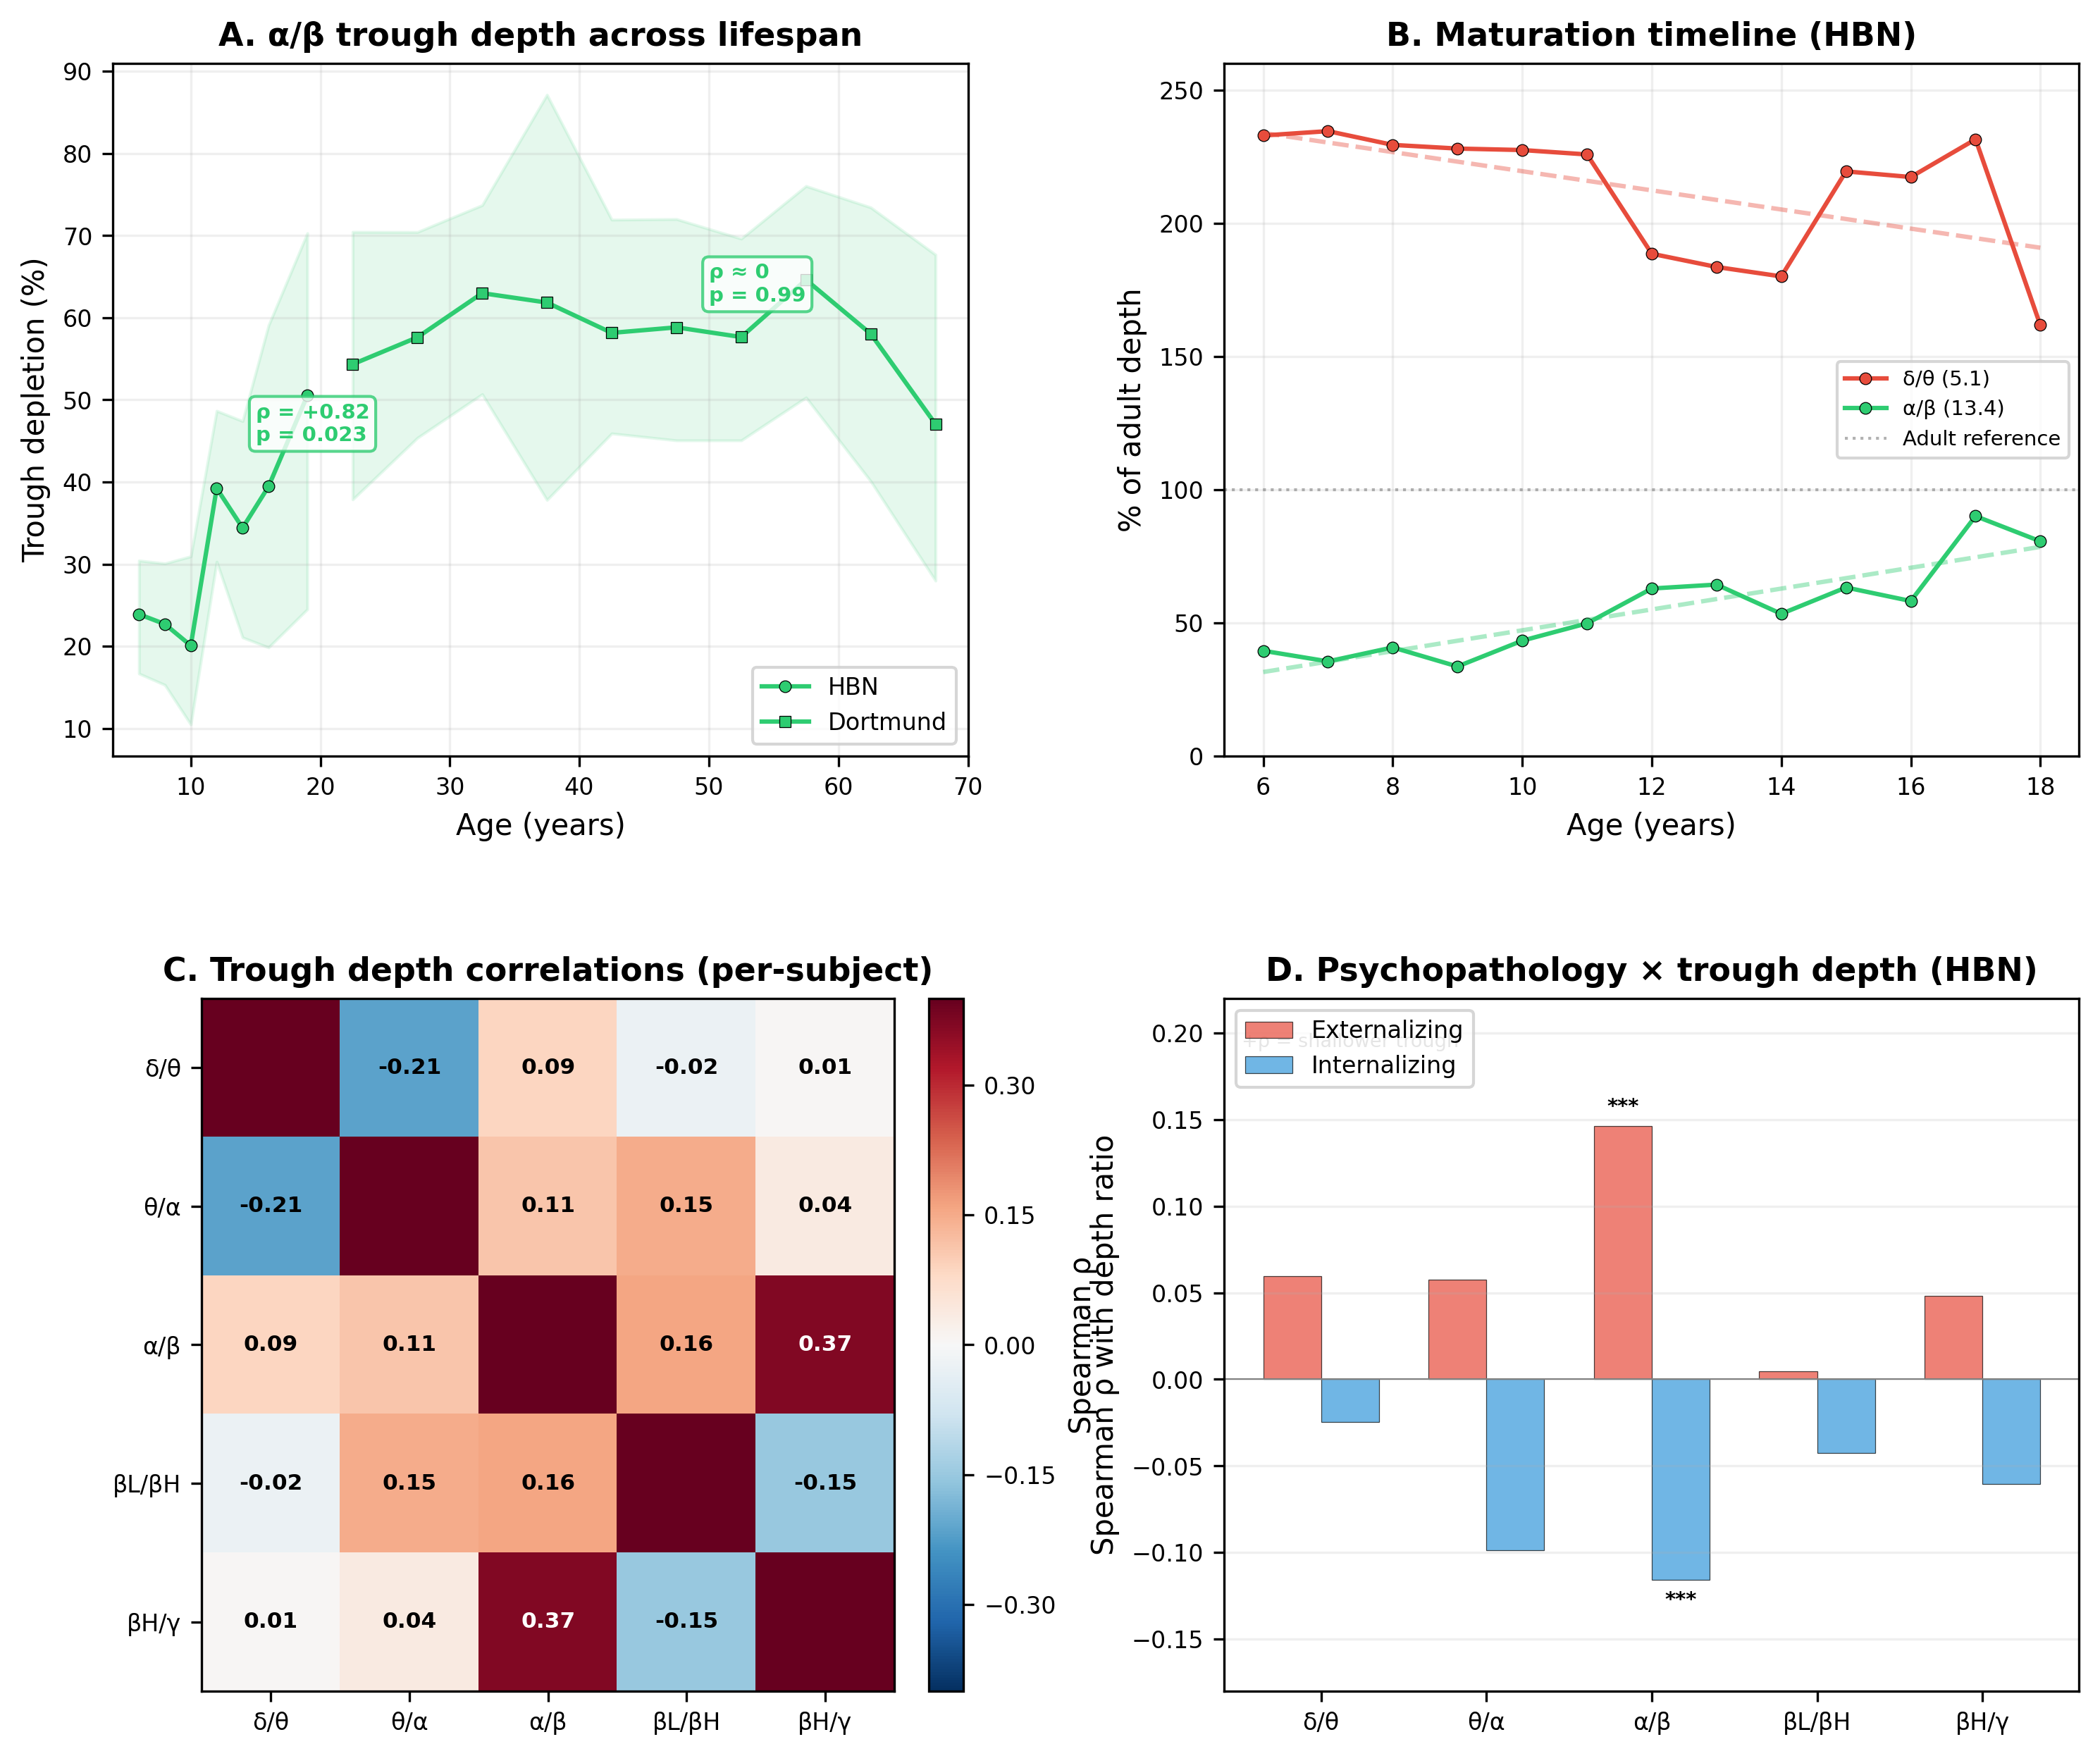
\includegraphics[width=\textwidth]{fig_trough_analyses.png}
\caption{\textbf{Trough depth analyses.} (A)~$\alpha$/$\beta$ trough depletion across the lifespan. Within HBN (ages 5--21), depletion increases monotonically ($\rho = +0.82$, $p = 0.023$); within Dortmund (ages 20--70), it is stable ($\rho \approx 0$, $p = 0.99$). Shaded bands: 95\% bootstrap CIs from 500 subject-level resamples per age bin. (B)~Differential maturation: the $\delta$/$\theta$ trough is over-deep in children ($>$200\% of adult depth) and regresses, while the $\alpha$/$\beta$ trough is immature ($\sim$40\%) and deepens on the PV+ interneuron maturation timeline. Dashed line: adult reference (Dortmund 25--55). (C)~Per-subject trough depth correlation matrix ($N = 1{,}738$). The five troughs are largely independent (mean off-diagonal $\rho = 0.053$); the $\alpha$/$\beta$--$\beta_H$/$\gamma$ cluster ($\rho = 0.37$) is the only substantial positive correlation. (D)~Psychopathology $\times$ trough depth in HBN ($N = 906$). Externalising and internalising symptoms push the $\alpha$/$\beta$ trough in opposite directions ($\rho = +0.146$ and $-0.116$, both FDR $q < 0.05$), consistent with GABA deficit and enhancement models respectively. ${}^{***}p < 0.001$.}
\label{fig:trough_analyses}
\end{figure}

\subsection{Boundaries Matter; Landmarks Do Not}

A conceptual clarification is warranted by the within-band profile results. Prior formulations of the $\phisym$-lattice framework \parencite{pletzer2010golden,kramer2023golden} have emphasized that noble-number frequency ratios suppress mode-locking between oscillators, suggesting that specific frequencies carry dynamical significance as anti-resonance points. The present data do not support this interpretation at the within-band level. Within-band frequency profiles are smooth and monotone---ascending ramps in most bands, a single mountain in alpha---with no evidence of fine structure, enrichment peaks, or depletion troughs at the positions predicted by noble-number arithmetic. Landmark frequencies, in this sense, do not matter.

What does matter is where the boundaries between bands are drawn. Log-spaced boundaries produce the simplest, most interpretable within-band spectral profiles. Misaligned boundaries---whether from using linear spacing or from individual $\fzero$ mismatch---import spectral content from adjacent bands, fragmenting what would otherwise be a clean profile and generating spurious enrichment and depletion patterns. The value of $\phisym$-scaling is coordinate-geometric rather than dynamical: it provides a partition of the frequency axis that minimizes cross-band leakage and thereby maximizes the discriminability of within-band oscillatory organization. A reviewer might note that the third-octave system ($r = 1.26$) achieves higher cross-dataset consistency ($r = 0.87$ vs.\ $0.79$ for the $\phisym$-lattice) in the boundary sweep. We optimize for profile simplicity rather than raw consistency because simplicity---the ability to describe within-band enrichment with a low-order polynomial---is what makes individual-differences metrics interpretable: a monotonic ramp has a meaningful slope, a mountain has a meaningful height, and both can be summarized by single numbers that predict cognition. High cross-dataset consistency of a \emph{complex} profile would be less useful, because the derived metrics would require more parameters and be harder to validate. The $\phisym$-lattice produces the simplest profiles ($R^2 = 0.968$) precisely because its boundaries fall where the spectral structure naturally transitions, yielding clean ramps and mountains rather than multi-modal shapes.

This reframing---from ``the brain computes with noble numbers'' to ``$\phisym$-scaling provides measurement-optimal boundaries for quantifying spectral differentiation''---is empirically more defensible and practically more consequential.

\subsection{Spectral Differentiation as a Novel Biomarker Class}

The spectral differentiation index introduced here occupies a distinct niche in the landscape of EEG-derived measures. It is not band power, which quantifies total energy without regard to internal structure. It is not the individual alpha frequency \parencite{klimesch1999eeg,grandy2013iaf,corcoran2018iaf}, which identifies a single peak location. It is not the aperiodic slope \parencite{donoghue2020fooof,voytek2015aperiodic}, which characterizes the background $1/f$ process. And it is not connectivity, which concerns relationships between spatially separated signals. Spectral differentiation measures something orthogonal to all of these: how organized the within-band peak distribution is, treating the histogram of individual-epoch spectral peaks as the object of inference.

A band with high spectral differentiation is one in which oscillatory epochs cluster tightly around a characteristic frequency, with few epochs straying into neighboring sub-bands. A band with low differentiation is one in which oscillatory activity is diffuse, irregular, or absent as a coherent phenomenon. Why should this matter for cognition? We suggest---as a hypothesis, not a demonstrated mechanism---that tighter frequency tuning supports more efficient neural communication through at least two routes. First, narrower frequency spread enables faster phase-locking between oscillating populations: two circuits operating at 19.5 $\pm$ 0.3 Hz can synchronize within a few cycles, while circuits operating at 19.5 $\pm$ 2.0 Hz require substantially longer to achieve coherence. Second, precise frequency tuning sharpens cross-frequency coupling: a 20 Hz signal couples to its 40 Hz harmonic more reliably than a smeared 17--23 Hz signal couples to anything in the gamma range. Both routes predict that high differentiation supports more efficient information transfer, consistent with the observed correlations with reasoning and executive function. This account is consistent with the ``communication through coherence'' framework \parencite{buzsaki2004neuronal} but remains speculative until tested with concurrent oscillatory and behavioral measures.

The cognitive correlate results underscore the biomarker potential. The core cognitive finding is that beta-low center depletion predicts reasoning ability ($\rho = -0.27$), survives both FDR correction and age partialing, and replicates under IRASA ($\rho = -0.29$, FDR $q < 0.02$). This cross-method replication anchors the cognitive story: it is not a FOOOF artefact. Beyond this anchor, an exploratory cognitive map generated by the framework identifies 31 FDR-surviving associations across four frequency bands and four cognitive domains in the LEMON dataset ($N = 203$). Earlier extraction pipelines with overly restrictive peak caps found zero cognitive FDR survivors in the same dataset---the 31 survivors emerge from correcting a systematic artefact, not from analytical degrees of freedom. Critically, cognitive associations survive IAF-partialing with only 23\% attenuation (vs.\ 47\% from age), confirming that spectral differentiation is not reducible to boundary misalignment. These effects are modest (peak $|\rho| \approx 0.27$, $R^2 \approx 7\%$ raw, $\approx 2\%$ unique after age), comparable to the strongest IAF--cognition effects in the literature ($|\rho| \approx 0.25$--$0.35$; \textcite{grandy2013iaf}). The broader 31-association map is FOOOF-specific and single-dataset; it should be regarded as a discovery-layer context for future replication, not a settled atlas.

Equally important are the informative nulls. Spectral differentiation is uninformative about personality traits (0/11,970 FDR in LEMON), medical and metabolic variables (0 FDR across $\sim$2,500 tests), and handedness (0 FDR in HBN and Dortmund). The contrast between 31 cognitive FDR survivors and zero personality survivors, in the same subjects with the same features, argues against the construct being a generic nuisance correlate or a signal artefact. It is selectively predictive of cognitive performance, not globally correlated with individual differences.

\subsection{An Inhibitory Circuit Hypothesis}
\label{sec:inhibitory}

The phase-locking and cross-frequency-coupling routes described above address the proximal mechanism by which differentiation supports cognition---tighter tuning enables faster synchronisation. A complementary question is what produces the tuning itself. This section consolidates the mechanistic evidence from the trough-depth analyses (Section~3.2), the psychopathology dissociation (Section~\ref{sec:psychopathology}), and the developmental trajectory (Sections~\ref{sec:development}--\ref{sec:lifespan}) into a unified hypothesis-generating framework. We suggest---as a hypothesis with testable pharmacological consequences, not a demonstrated result---that spectral differentiation is primarily a readout of PV+ fast-spiking interneuron circuit integrity, expressed most clearly at the $\alpha$/$\beta$ boundary. A brain with high spectral differentiation has sharp inhibitory boundaries that confine oscillatory peaks to well-defined spectral territories; a brain with low differentiation has weak or immature inhibitory boundaries that allow spectral energy to smear across the frequency axis.

This interpretation connects four otherwise disparate findings. First, the externalising--internalising psychopathology dissociation (Section~\ref{sec:psychopathology}): externalising symptoms (associated with GABAergic deficits in ADHD; \textcite{edden2012gaba}) are associated with flatter within-band profiles \emph{and} a shallower $\alpha$/$\beta$ trough, while internalising symptoms are associated with more concentrated upper-alpha enrichment \emph{and} a deeper $\alpha$/$\beta$ trough---the direction expected if anxious hypervigilance reflects enhanced, not diminished, inhibitory tone. Second, the personality null (Section~\ref{sec:nulls}): personality dimensions lack established GABAergic substrates, so a readout of inhibitory circuit integrity should be silent for personality, which it is (0/11,970 FDR). Third, the cognitive results operate at the within-band level, not the boundary level: supplementary analyses found only 1/40 FDR-surviving associations between per-subject trough depth and cognitive scores in LEMON, versus 31 for within-band enrichment. This distinction is expected if the cognitively relevant output of inhibitory circuits is peak \emph{organisation}---how precisely oscillatory activity is tuned within each band---rather than gap \emph{depth} per se. Fourth, the developmental trajectory of the $\alpha$/$\beta$ trough (Section~3.2) directly tracks PV+ maturation.

These predictions are jointly testable. Table~\ref{tab:pharmacological} enumerates three pharmacological agents, each targeting a different component of the proposed mechanism. The pattern of selective effects on the $\alpha$/$\beta$ trough (predicted to respond to GABAergic agents) versus the $\delta$/$\theta$ trough (predicted to be unaffected, since it is generator-dominated) would directly discriminate the inhibitory model from alternatives. A complementary correlational test: individual differences in spectral differentiation should correlate with cortical GABA concentration measured by magnetic resonance spectroscopy (MRS); no MRS-EEG study has yet examined within-band peak distributions. The inhibitory interpretation is not uniquely determined by the present data---variation in excitatory mechanisms (e.g., NMDA receptor kinetics) could produce similar patterns---but the GABAergic account is distinguished by its parsimony (a single mechanism class explains both the trough depth hierarchy and the psychopathology dissociation) and its experimental accessibility.

\begin{table}[h]
\centering
\caption{Predicted pharmacological dissociations under the GABAergic inhibitory model. Each agent targets a different component of the proposed mechanism; the pattern of selective effects on the $\alpha$/$\beta$ versus $\delta$/$\theta$ trough distinguishes the inhibitory model from alternatives. None of these predictions has been tested.}
\label{tab:pharmacological}
\begin{tabular}{l l l l l}
\toprule
Agent & Target & $\alpha$/$\beta$ trough & $\delta$/$\theta$ trough & Distinguishes \\
\midrule
Ethosuximide & T-type Ca$^{2+}$ & No change & No change & Null on both = inhibitory model \\
Benzodiazepine & GABA$_\text{A}$ PAM & Deepens, shifts down & No change & $\alpha$/$\beta$-only = PV+ model \\
Tiagabine & GABA reuptake & Broadens & No change & $\alpha$/$\beta$-only = two-class model \\
\bottomrule
\end{tabular}
\end{table}

\subsection{Spectral Differentiation and the Inverted-U of Cognitive Aging}

If spectral differentiation tracks the inverted-U of neural differentiation across the lifespan \parencite{li2004dedifferentiation}, it would provide the first frequency-domain EEG measure with a principled connection to this framework. The de-differentiation hypothesis holds that neural representations become more distinct and specialized through childhood and early adulthood, then progressively lose specificity in aging, with this loss mediating much of the cognitive decline observed in older adults.

The cross-sectional HBN developmental data are consistent with the ascending limb: spectral differentiation increases from childhood through adolescence, attributable to the progressive maturation of myelination, synaptic pruning, and inhibitory interneuron populations that together sharpen the frequency tuning of cortical circuits. Of these processes, the PV+ inhibitory interneuron trajectory is the most temporally specific. The $\alpha$/$\beta$ trough reaches 50\% of its adult depth at age 12 and 75--90\% by age 17 (Section~3.2), coinciding with perineuronal net consolidation that stabilises PV+ fast-spiking function \parencite{hensch2005critical}. The distinction between \emph{immature} troughs ($\alpha$/$\beta$, $\theta$/$\alpha$) that deepen during development and \emph{over-mature} troughs ($\delta$/$\theta$, $\beta_L$/$\beta_H$) that regress toward adult levels (Section~3.2) suggests that the ascending limb of the inverted-U has two components: progressive sharpening of inhibitory boundaries and simultaneous recession of generator-dominated boundaries that were over-deep in childhood. LEMON adult data then show the expected positive relationship between differentiation and cognitive performance. The Dortmund aging data show the descending limb: the same features that increase during development decrease during aging, with 28 of 31 cross-dataset features showing opposite signs. At the trough level, the $\theta$/$\alpha$ boundary shallows significantly during aging ($\rho = -0.81$, $p = 0.005$ within Dortmund), and the $\beta_L$/$\beta_H$ trough inverts from depletion to enrichment ($\rho = -0.92$, $p = 0.0002$), suggesting progressive degradation of boundary structure in the second half of life---consistent with the known vulnerability of PV+ interneurons to oxidative stress and aging-related loss.

If spectral differentiation is the oscillatory substrate of cognitive de-differentiation, then aging populations should show systematically lower differentiation scores, and the magnitude of this decline should predict the degree of cognitive impairment. This prediction is testable in existing datasets such as TDBRAIN or Cambridge Centre for Ageing and Neuroscience (Cam-CAN). However, as noted in Section~\ref{sec:lifespan}, the inverted-U trajectory is driven entirely by the cross-cohort splice between HBN and Dortmund rather than by a within-cohort turning point, and longitudinal data spanning childhood through middle age would be needed to confirm whether the vertex at $\sim$33--35 years is genuine or an artefact of the cross-sectional design.

\subsection{Corrections to Prior Work}

Scientific progress occasionally requires explicit correction of one's own prior claims, and this paper presents several. \textcite{lacy2026frontiers} reported two findings as universal features of the $\phisym$-lattice framework: aggregate boundary depletion (spectral troughs co-locating with band boundaries across all bands) and Noble$_1$ enrichment (peaks clustering near the first noble-number landmark within each band). Both claims were supported by statistically significant results in that analysis.

The present v3 analysis demonstrates that both findings were artifacts of the extraction pipeline. The aggregate boundary depletion was driven by a $\fzero$ mismatch that wrapped peaks into incorrect Voronoi bins, most consequentially reversing the beta-low boundary from $+101\%$ to $-33\%$. The Noble$_1$ enrichment is real but alpha-specific---it does not generalize to theta, beta-low, beta-high, or gamma (all show Noble$_1$ $\approx 0\%$). The aggregate effect reported in the Frontiers paper was an average over five bands in which one band (alpha) showed strong enrichment and four showed null, producing a misleadingly positive aggregate.

Earlier extraction pipelines with overly restrictive peak caps produced zero cognitive FDR survivors and negative test--retest ICCs ($\text{ICC} < 0$) for spectral differentiation. The 31 FDR survivors and strongly positive ICCs ($0.42$--$0.75$) reported here emerge from the same datasets with corrected extraction parameters, demonstrating that the prior null results were methodological artifacts rather than genuine absence of signal.

The framework introduced in \textcite{lacy2026frontiers} is confirmed as a measurement framework by these results; the specific empirical claims it advanced required correction. Three methodological corrections substantially change the enrichment landscape and reveal previously hidden cognitive, developmental, and clinical associations.

\subsection{Robust and Provisional Claims}

For clarity, we distinguish claims that are strongly supported by the present evidence from those that remain provisional. \textbf{Robust claims}: logarithmic frequency scaling ($\Delta$BIC $> 50$); five real density troughs confirmed by the aperiodic null ($p < 0.0001$) and recovered in 100\% of subject-level bootstraps; $\phisym$ as the best-supported named global boundary constant tested (bootstrap 95\% CI [1.609, 1.623]); the $\phisym$-lattice as a measurement-optimal coordinate system for profile simplicity ($R^2 = 0.968$; boundaries within 2\% of locally optimal positions); the alpha mountain and upper-octave depletion cascade (11/13 cross-dataset consistency under FOOOF, replicated under IRASA); the beta-high descending ramp (method-independent, 13/13 cross-dataset consistency under IRASA); the top cognitive association---beta-low center depletion as a predictor of reasoning---replicating across methods (FDR-significant under both FOOOF and IRASA), though the breadth of the cognitive map (31 FDR survivors) is FOOOF-specific; the developmental inverted-U trajectory (68 FDR survivors under both methods); 5-year test--retest reliability of beta-low spectral differentiation (ICC $= 0.75$). \textbf{Provisional claims}: exact $\phisym$ ontology (the CI contains $\phisym$ but also nearby values; local boundary ratios are heterogeneous); theta enrichment geometry (method-dependent, inverted under IRASA); gamma within-band architecture (weak cross-dataset consistency, scalp EEG contamination); the specific cognitive effect sizes (single-dataset, modest $\rho$); the vertex of the inverted-U at 33--35 years (cross-sectional splice); the PV+ inhibitory interpretation of the $\alpha$/$\beta$ trough and spectral differentiation (developmental and psychopathological correlations consistent with PV+ maturation, but post hoc and without direct neurochemical evidence; pharmacological and MRS predictions untested); and the two-class trough mechanism model (inhibitory-boundary versus generator-dominated; based on developmental trajectory classification, not direct mechanism measurement).

\subsection{Limitations}
\label{sec:limitations}

Several limitations constrain the conclusions drawn here. First, the cognitive correlate analyses rely on a single dataset (LEMON, $N = 203$) and require independent replication before the 31 FDR-surviving associations can be regarded as established. At $N = 203$, a two-tailed Spearman correlation has approximately 80\% power to detect $|\rho| \geq 0.20$ at $\alpha = 0.05$ for a single test; however, FDR correction across 720 simultaneous tests raises the effective detection threshold, meaning that true associations weaker than the observed $|\rho| \approx 0.25$ are likely missed. The 31 FDR survivors should therefore be regarded as a lower bound on the number of genuine associations rather than an exhaustive catalogue. Sample size, demographic homogeneity, and task battery all limit generalizability.

Second, the band boundaries employed throughout are defined at the population level. Individual $\fzero$ values span 8--13 Hz in healthy adults \parencite{klimesch1999eeg,grandy2013iaf}, sufficient to cause boundary misalignment. The IAF-partialing analysis (Section~\ref{sec:cognitive}) demonstrates that this confound is not the primary driver of the cognitive results: IAF-partialing attenuates correlations by only 23\% (and adds only 4 percentage points beyond age alone, reflecting IAF-age collinearity), with 31/46 strong features surviving. Nevertheless, individual-specific coordinate systems anchored to each subject's $\fzero$ remain the principled approach and should improve sensitivity, particularly for beta-low features where the alpha mountain's flank determines ramp position.

Third, the subject-level bootstrap discriminates among the named candidate constants ($\phisym$, $e-1$, $\sqrt{2}$, etc.) by showing that only $\phisym$ lies within the 95\% CI for the global inter-trough ratio. However, it does not establish that $\phisym$ is the exact value---the CI [1.609, 1.623] also contains nearby non-named values---nor does it imply exact local $\phisym$-spacing at every boundary, since individual boundary ratios remain heterogeneous (1.36--1.89). The bootstrap resolves the named-constant question but not the deeper question of whether the ratio is exactly $\phisym$ or merely a biophysical constant that happens to fall near 1.618.

Fourth, the developmental data from HBN are cross-sectional. Longitudinal tracking of spectral differentiation from childhood through adulthood would be required to establish the causal direction of the differentiation-cognition relationship and to test the inverted-U prediction directly.

Fifth, all primary analyses rely on FOOOF/specparam for aperiodic-periodic separation. The IRASA replication (Section~\ref{sec:irasa}) demonstrates selective method-independence: beta-high enrichment, the top cognitive association, and the developmental trajectory replicate under a fundamentally different non-parametric approach, while theta and gamma remain method-sensitive. The broader cognitive map (31 FDR survivors) is FOOOF-specific; a peak-yield subsample test (Section~\ref{sec:irasa}) attributes this primarily to IRASA's lower per-subject peak yield in the bands carrying the strongest cognitive signal. The strongest features are not artefacts of the parametric approach; the broader map requires either FOOOF's yield or larger samples.

\subsection{Future Directions}

The most immediate priority is the construction of individual-specific frequency coordinate systems. If each subject's band boundaries are shifted proportionally to their $\fzero$---so that the theta-alpha boundary falls at $\fzero / \phisym$ regardless of whether $\fzero = 9$ Hz or $\fzero = 11$ Hz---the boundary misalignment artifacts are eliminated by construction. This approach, which we term IAF-anchored spectral differentiation, should be the default in future work \parencite{corcoran2018iaf,klimesch1999eeg}.

Source-space analysis represents a second priority. MEG, ECoG, and high-density EEG with source modeling would allow spectral differentiation to be applied to specific cortical and subcortical structures, testing whether cognitive correlates show regional specificity and resolving the gamma contamination concern.

Clinical translation offers a third direction. Neurodegenerative diseases are associated with progressive disruption of thalamocortical circuits \parencite{klimesch2018frequency}, and the two-mechanism model predicts that alpha mountain flattening should be among the earliest spectral signatures of thalamic pathology.

Pharmacological and neurochemical validation of the inhibitory model represents a fourth priority. The predictions in Table~\ref{tab:pharmacological} specify a crossover design in which ethosuximide, a benzodiazepine, and tiagabine are administered to healthy volunteers, with pre- and post-drug spectral differentiation and trough depth computed from resting EEG. The differential prediction---GABAergic agents affecting the $\alpha$/$\beta$ trough but not the $\delta$/$\theta$ trough---directly tests the two-class mechanism model. An MRS-EEG study correlating individual cortical GABA concentration with spectral differentiation would provide complementary correlational evidence and represents the most immediately feasible test of the framework, given that MRS-GABA protocols are established \parencite{edden2012gaba} and could be applied to existing multimodal datasets such as Cam-CAN.

Finally, the neurofeedback literature has established that oscillatory power can be upregulated through closed-loop training, but has not examined whether spectral differentiation---the organization of oscillatory activity, as distinct from its magnitude---can be similarly targeted. If the cognitive benefits of neurofeedback derive from improved spectral organization rather than increased power, then differentiation-targeted protocols should outperform power-targeted ones.


%==============================================================================
% METHODS
%==============================================================================
\section{Methods}
\label{sec:methods}

\subsection{Datasets}
\label{sec:datasets}

We assembled five publicly available resting-state EEG datasets comprising 2,097 participants and nine eyes-closed (EC) recording conditions (Table~\ref{tab:datasets}).

\begin{table}[htbp]
\centering
\caption{EEG datasets included in the analysis. N = number of subjects contributing at least one valid EC resting-state recording. HBN releases R1--R6 (R5 excluded due to artefact contamination) are treated as independent replications within the paediatric cohort.}
\label{tab:datasets}
\begin{tabular}{llrrll}
\toprule
\textbf{Dataset} & \textbf{N} & \textbf{Channels} & \textbf{Age (years)} & \textbf{Country} & \textbf{Conditions} \\
\midrule
EEGMMIDB & 109 & 64 & adult & USA & 14 runs pooled \\
LEMON & 203 & 59 & 20--77 & Germany & EC, EO \\
Dortmund & 608 & 64 & 18--70 & Germany & EC/EO $\times$ pre/post $\times$ ses-1/ses-2 \\
CHBMP & 250 & 62--120 & adult & Cuba & EC \\
HBN R1--R6 & 927 & 128 & 5--21 & USA & Mixed resting \\
\midrule
\textbf{Total} & \textbf{2,097} & & & & \textbf{9 EC conditions} \\
\bottomrule
\end{tabular}
\end{table}

The \textbf{EEG Motor Movement/Imagery Database (EEGMMIDB)} comprises 109 healthy adults recorded with a 64-channel system at 160 Hz \parencite{goldberger2000physiobank,schalk2004bci2000}. Subjects performed fourteen one-minute runs covering rest and motor imagery tasks; all runs were pooled per subject.

The \textbf{LEMON} (Leipzig Study for Mind-Body-Emotion Interactions) dataset comprises 203 healthy adults (ages 20--77) recorded with 59 channels at 2500 Hz \parencite{babayan2019lemon}. Paired EC and EO resting-state blocks ($\approx$15 minutes each) and a neuropsychological battery including the Leistungsprüfsystem (LPS), Test of Attentional Performance (TAP), Regensburger Wortflüssigkeits-Test (RWT), and Trail Making Test (TMT) make LEMON the primary cognitive-correlates dataset.

The \textbf{Dortmund EEG dataset} is a longitudinal sample of 608 healthy German adults (ages 18--70) recorded at 64 channels, with a subset of $N = 208$ returning approximately five years later \parencite{vossen2015dortmund}. The longitudinal subsample provides five-year test--retest reliability estimates.

The \textbf{Cuban Human Brain Mapping Project (CHBMP)} provides EC resting-state recordings from 250 healthy Cuban adults recorded at 62--120 channels.

The \textbf{Healthy Brain Network (HBN)} dataset \parencite{alexander2017hbn} is a paediatric community sample of 927 participants (ages 5--21) from the New York City area, recorded at 128 channels. Five independent data releases (R1, R2, R3, R4, R6; R5 excluded due to artefact contamination) were analysed to test cross-sample reproducibility. HBN includes the Child Behavior Checklist (CBCL) for psychopathology measures.

\subsection{EEG Preprocessing and Spectral Peak Extraction}
\label{sec:extraction}

All datasets were processed through a common v3 pipeline. Raw recordings were bandpass filtered from 1 to 59~Hz with a zero-phase fourth-order Butterworth filter. European recordings (LEMON and Dortmund) received an additional 50~Hz notch filter ($Q = 30$) to suppress mains-frequency contamination. All recordings were resampled to 250~Hz.

Spectral peaks were extracted using the FOOOF/specparam framework \parencite{donoghue2020fooof}, which models each power spectrum as the sum of an aperiodic $1/f$-like component and Gaussian peaks. Adaptive Welch windowing with a minimum segment length of 2500 samples (10~s at 250~Hz) yielded frequency resolution $\Delta f = 0.1$~Hz. The bandwidth floor was set to $2 \times \Delta f = 0.2$~Hz.

Four fitting ranges were applied sequentially:
\begin{enumerate}
    \item \textbf{Merged theta--alpha}: 4.70--12.30~Hz, single aperiodic component.
    \item \textbf{Beta-low}: 12.30--19.90~Hz.
    \item \textbf{Beta-high}: 19.90--32.19~Hz.
    \item \textbf{Gamma}: 32.19--52.09~Hz.
\end{enumerate}

Global specparam parameters: \texttt{peak\_threshold} $= 0.001$, \texttt{max\_n\_peaks} $= 15$, \texttt{min\_peak\_height} $= 0.0001$. Each peak was retained only if $R^2 \geq 0.70$ (median $R^2 = 0.931$ across all retained peaks). Each peak was characterised by centre frequency, power, bandwidth, $R^2$, and $\phisym$-octave assignment. After power filtering (Section~\ref{sec:power_filter}), the final dataset comprised 4,572,489 peaks from an initial 9,132,221.

\subsubsection{Three Methodological Corrections}
\label{sec:methods_corrections}

\paragraph{Correction 1: $\fzero$ alignment.}
Peaks are assigned to bands via the normalised coordinate:
\begin{equation}
u = \left(\frac{\log(f / \fzero)}{\log \phisym}\right) \bmod 1,
\label{eq:u_coord}
\end{equation}
where $\fzero = 7.60$~Hz. A prior 3\% mismatch between extraction ($\fzero = 7.83$~Hz) and enrichment coordinates ($\fzero = 7.60$~Hz) caused boundary-wrapping artifacts. Aligning both to $\fzero = 7.60$~Hz eliminated five sign reversals.

\paragraph{Correction 2: Hz-weighted null.}
Under a Hz-uniform detection process, the expected count in Voronoi bin $i$ with $u$-edges $[u_L, u_R]$ is:
\begin{equation}
\hat{E}_i = \frac{\phisym^{u_R} - \phisym^{u_L}}{\phisym - 1} \cdot N,
\label{eq:hz_weighted_null}
\end{equation}
where $N$ is total peaks in the band. Enrichment is:
\begin{equation}
\text{Enr}_i = \left(\frac{n_i}{\hat{E}_i} - 1\right) \times 100\%.
\label{eq:enrichment}
\end{equation}

\paragraph{Correction 3: Merged theta--alpha fit.}
Separate FOOOF fits for theta and alpha created a 15$\times$ step discontinuity in peak density at $\fzero$. Merging into a single fit (4.70--12.30~Hz) eliminated this artifact ($r = 0.913$ with separate alpha profile; $r = 0.200$ with separate theta, confirming the theta profile was dominated by the boundary artifact).

\subsubsection{Power Filtering}
\label{sec:power_filter}

Permissive extraction (\texttt{peak\_threshold} $= 0.001$) retained virtually all supra-background features. Analysis-time filtering then kept the top 50\% of peaks by power within each band per subject. This ``permissive extraction + analysis-time filtering'' strategy outperformed strict-threshold extraction on all validation metrics.

\subsubsection{Parameter Validation}
\label{sec:param_validation}

A 48-configuration parameter sweep on EEGMMIDB (GCP c2d-standard-32, $\sim$30 minutes total) factorially combined \texttt{peak\_threshold} $\in \{0.001, 0.01, 0.1, 2.0\}$, \texttt{min\_peak\_height} $\in \{0.00, 0.05, 0.10, 0.15, 0.20\}$, \texttt{max\_n\_peaks} $\in \{5, 8, 12, 15, 20\}$, and adaptive versus fixed Welch segmentation. Only \texttt{max\_n\_peaks} materially affected enrichment (inflection at 12, matching the 12 Voronoi positions). The production value of 15 was chosen for stable per-subject estimates.

\subsection{Log-Frequency Scaling Tests}
\label{sec:scaling_methods}

Seven tests evaluated whether the peak distribution is better described in log-frequency or linear-frequency space, and whether the inter-trough ratio is robust to the dependence structure of the data.

\textbf{Test 1: KDE density estimation.} Peak frequencies were pooled ($N = 4{,}572{,}489$) and Gaussian KDE applied in both linear-Hz and log-Hz spaces ($h = 0.02$). Local minima (density troughs) were identified as empirical band boundaries.

\textbf{Test 2: BIC model comparison.} Empirical boundary and centre frequencies were fitted by geometric series $f_k = \fzero \times r^k$ for seven fixed ratios ($\phisym$, $e-1$, $\sqrt{3}$, 2, $e$, $2^{1/3}$, $\sqrt{2}$), a free-ratio model (2 parameters), and linear-Hz spacing (2 parameters). BIC $= n \ln(\text{SSE}/n) + k \ln n$.

\textbf{Test 3: Polynomial BIC.} Peak frequencies were histogrammed in 100 equal-width bins in linear-Hz and log-Hz. Polynomial BIC (degrees 2--6) compared description parsimony.

\textbf{Test 4: Per-dataset replication.} Tests 1--3 were repeated independently on each of 9 datasets. One-sample $t$-tests on log-transformed ratios tested $H_0: \mu_{\log r} = \log r_\text{candidate}$.

\textbf{Test 5: Smoothing stability.} Trough locations were tracked across 30 smoothing bandwidths ($\sigma = 2$--30 bins on a 1000-bin log-frequency histogram). A trough was ``stable'' if present in $>50\%$ of smoothings.

\textbf{Test 6: Aperiodic null.} 200 Poisson surrogates were drawn from a heavily smoothed ($\sigma = 40$ bins) version of the real log-frequency histogram, preserving the $1/f$ envelope while destroying band structure. Trough depths were compared between real data and surrogates.

\textbf{Test 7: Subject-level bootstrap.} To account for the non-independence of peaks nested within subjects, 1,000 bootstrap resamples were drawn at the \emph{subject} level, stratified by dataset (preserving the 9-dataset composition at each iteration). For each resample, the full trough-detection pipeline (histogram $\to$ smoothing $\to$ peak-finding) was re-run from scratch on the pooled resampled peaks. Trough positions were matched to reference troughs algorithmically by nearest-neighbour assignment in log-frequency space (maximum distance: 0.3 log-Hz, corresponding to $\approx$35\% in Hz). The global inter-trough geometric mean ratio was computed for each bootstrap iteration. Confidence intervals were derived as the 2.5th and 97.5th percentiles. Two-sided bootstrap $p$-values for candidate constants were computed as $p = 2 \times \min(F(\theta), 1 - F(\theta))$, where $F(\theta)$ is the proportion of bootstrap replicates at or below the candidate value $\theta$.

\subsection{Boundary Sweep}
\label{sec:sweep_methods}

A $36 \times 36$ grid of $(\fzero, r)$ pairs spanning $\fzero \in [6.0, 9.5]$~Hz and $r \in [1.3, 2.3]$ was evaluated. For each coordinate system, band boundaries were placed at $\fzero \cdot r^n$. The normalised intra-band coordinate is:
\begin{equation}
u = \frac{\log(f / f_\text{lower})}{\log r},
\end{equation}
which is invariant to the choice of logarithm base. Within each band, peaks were binned into 12 equal-width $u$-bins with Hz-weighted expected counts (Equation~\ref{eq:hz_weighted_null}).

Three metrics were evaluated: \textbf{profile simplicity} (mean $R^2$ of best linear/quadratic fit across bands), \textbf{cross-dataset consistency} (mean pairwise Pearson $r$ of enrichment vectors across 9 datasets), and \textbf{band independence} (mean $|r|$ between adjacent bands' profiles, inverted). A boundary-slide analysis independently varied each boundary $\pm 25\%$ while holding others fixed.

\subsection{Within-Band Coordinate Tests}
\label{sec:within_methods}

Five tests evaluated within-band structure under the $(\fzero = 7.60, r = \phisym)$ system, using 200-bin Hz-corrected enrichment profiles.

\textbf{Test 1: Scaling comparison.} Five frequency scales (log, linear, ERB, mel, $\sqrt{\text{Hz}}$) were compared by polynomial $R^2$.

\textbf{Test 2: Landmark capture.} Voronoi $R^2$ of 12 $\phisym$-positions versus 12 equal-spaced, 12 rational, and 1000 random position sets.

\textbf{Test 3: Feature alignment.} Mean distance from enrichment extrema to nearest $\phisym$-position; 5000-permutation null.

\textbf{Test 4: Periodicity.} Autocorrelation of enrichment profiles at lags corresponding to $\phisym^{-k}$, $1/2$, $1/3$.

\textbf{Test 5: Noble vs.\ rational.} Enrichment at noble numbers versus simple rationals; 5000-permutation test.

\subsection{Voronoi Enrichment}
\label{sec:voronoi}

Twelve degree-6 positions per $\phisym$-octave were used as Voronoi landmarks:
\begin{equation}
\mathbf{u} = \{0,\; \phisym^{-6},\; \phisym^{-5},\; \phisym^{-4},\; \phisym^{-3},\; \phisym^{-2},\; 0.5,\; \phisym^{-1},\; 1-\phisym^{-3},\; 1-\phisym^{-4},\; 1-\phisym^{-5},\; 1-\phisym^{-6}\}.
\end{equation}

Each peak was assigned to its nearest position (circular distance). The boundary position ($u = 0$) was split into boundary\_lo and boundary\_hi for analysis of $\fzero$-convergence effects. Hz-weighted expected counts were computed per Equation~\ref{eq:hz_weighted_null}.

Six derived metrics summarise each band's profile: \textbf{mountain} (Noble$_1$ $-$ boundary), \textbf{ushape} (mean edges $-$ attractor), \textbf{peak\_height} (Noble$_1$ $-$ attractor), \textbf{ramp\_depth} (inv\_noble$_4$ $-$ noble$_4$), \textbf{center\_depletion} (attractor $-$ mean lower interior), and \textbf{asymmetry} (mean upper interior $-$ mean lower interior).

\subsection{Individual-Differences Analyses}
\label{sec:individual_diffs}

Per-subject enrichment profiles were computed for subjects with $\geq 30$ peaks per band after power filtering. Associations with continuous variables were quantified by Spearman $\rho$, corrected by Benjamini--Hochberg FDR ($q < 0.05$) within each analysis family. Age-partialed correlations used van der Waerden normal scores. Test--retest reliability (Dortmund longitudinal, $N = 208$) was estimated by ICC(2,1) (two-way random, absolute agreement, single measures).

\subsection{Computational Infrastructure}
\label{sec:infrastructure}

Peak extraction was parallelised on Google Cloud Platform (c2d-standard-32 VMs, custom image). Each dataset was processed as: VM spawn $\to$ GCS data copy $\to$ parallel per-subject extraction (28 cores) $\to$ results push $\to$ VM deletion ($\sim$5 minutes per dataset). The 48-configuration parameter sweep completed in $\sim$30 minutes. All code: Python 3.10 (NumPy 1.26, SciPy 1.11, pandas 2.1, specparam 1.0). All analysis code and extracted peak CSVs are archived on GCS.

\subsection{Ethics Statement}
\label{sec:ethics}

This study is a secondary analysis of publicly available, de-identified EEG datasets. All original studies obtained institutional ethics approval and informed consent from participants (or their guardians, in the case of HBN minors) prior to data collection and public release. No additional ethics approval was required for the present analyses of these de-identified data.

\subsection{Use of Artificial Intelligence Tools}
\label{sec:ai_disclosure}

Anthropic Claude Code (Opus 4.6) was used to assist with data analysis pipeline development and manuscript preparation. Anthropic Claude (Opus 4.6, chat) and OpenAI ChatGPT (5.4) were used as reviewers to check for consistency, clarity, errors, and omissions. All AI-generated content was reviewed, verified, and edited by the author, who takes full responsibility for the accuracy and integrity of the work.


%==============================================================================
% DATA AVAILABILITY
%==============================================================================
\section*{Data and Code Availability}

Extracted spectral peaks (14.7 million FOOOF and 11.7 million IRASA peaks), per-subject enrichment profiles, subject demographics, and all statistical analysis outputs are available on Dryad (\url{https://doi.org/10.5061/dryad.1vhhmgr8t}). All analysis code is available at \url{https://github.com/neurokinetikz/research} under the MIT License. Raw EEG data are publicly available from their original sources: EEGMMIDB (PhysioNet, \url{https://physionet.org/content/eegmmidb/}; \cite{goldberger2000physiobank}), LEMON (Max Planck Institute, \url{http://fcon_1000.projects.nitrc.org/indi/retro/MPI_LEMON.html}; \cite{babayan2019lemon}), HBN (Child Mind Institute, \url{http://fcon_1000.projects.nitrc.org/indi/cmi_healthy_brain_network/}; \cite{alexander2017hbn}), Dortmund Vital Study (OpenNeuro, \url{https://doi.org/10.18112/openneuro.ds005385.v1.0.3}), and CHBMP (CAN-BIND data sharing portal). CHBMP-derived data are not included in the Dryad package due to its CC BY-NC-SA license but can be reproduced from the source data using the provided extraction code. LEMON cognitive test scores and HBN CBCL psychopathology scores are available from their respective data portals under the original data use agreements.

%==============================================================================
% ACKNOWLEDGMENTS
%==============================================================================
\section*{Acknowledgments}

The author thanks the teams behind the publicly available datasets that made this work possible: the PhysioNet EEGMMIDB \parencite{goldberger2000physiobank}, the MPI Leipzig Mind-Brain-Body LEMON study \parencite{babayan2019lemon}, the Child Mind Institute Healthy Brain Network \parencite{alexander2017hbn}, the Dortmund Vital Study, and the Canadian Biomarker Integration Network for Depression (CAN-BIND) CHBMP. Computational resources were provided by Google Cloud Platform.

%==============================================================================
% AUTHOR CONTRIBUTIONS
%==============================================================================
\section*{Author Contributions}

Michael Lacy: Conceptualization, Data curation, Formal analysis, Investigation, Methodology, Software, Validation, Visualization, Writing -- original draft, Writing -- review \& editing.

%==============================================================================
% COMPETING INTERESTS
%==============================================================================
\section*{Competing Interests}

The author declares no competing interests.

%==============================================================================
% FUNDING
%==============================================================================
\section*{Funding}

No external funding was received for this work.

%==============================================================================
% REFERENCES
%==============================================================================
\newpage
\printbibliography

\end{document}
